\documentclass[12pt,a4paper]{article}

\usepackage{amsmath}
\usepackage{graphicx}
\usepackage{booktabs}
\usepackage{siunitx}
\graphicspath{{../../output/benchmarks/campaign-runs/formal-1/warm/repeat-1/analysis/benchmark-report-1/}}
\usepackage{tabularx}
\usepackage{xurl}
\usepackage{microtype}
\usepackage{array}
\usepackage{caption}
\usepackage{verbatim}
\usepackage[toc,page]{appendix}

% Set up BibLaTeX efficiently
\usepackage[numbers,sort&compress]{natbib}

% For placing figures exactly where they are declared
\usepackage{float}
\usepackage[section]{placeins}

\usepackage{fancyhdr}
\fancyhf{}
\renewcommand{\headrulewidth}{0.5pt}
\renewcommand{\footrulewidth}{0.5pt}
\setlength{\headheight}{15pt}
\fancyhead[L]{Anna Kudrych}
\fancyhead[R]{SOC10101 - Honours Project}
\fancyfoot[L]{}
\fancyfoot[C]{\thepage}

\usepackage[hidelinks]{hyperref}

\begin{document}
\pagenumbering{roman}

% \input{./Dissertation-Title.tex}
% \input{./Dissertation-Dec.tex}
% \pagebreak
% \input{./Dissertation-DP.tex}
% \pagebreak

\begin{abstract}
Post-quantum cryptography standards have been published, but organisations face a practical question with no empirical answer in the existing literature: what does it actually cost, in latency and storage, to integrate these algorithms into a complete cloud file-signing workflow rather than a standalone benchmark? This study fills this gap by implementing and benchmarking a security-hardened Rust microservice prototype that models a more realistic backend signing pipeline comprising an API gateway, a dedicated hashing service, a manifest builder, a PostgreSQL database, and a MinIO object store.

A formal Phase 1 campaign executes 63\,000 measured runs across 630 conditions - seven signature profiles (RSA-PSS, ECDSA, EdDSA, HMAC-SHA256, ML-DSA,
SLH-DSA, FN-DSA), three hash algorithms (SHA-256, BLAKE3, Keccak-256), five payload sizes (10~KB-50~MB), and six workflow scenarios - to produce
decision-grade performance data at 95\% bootstrap confidence~\cite{efron1979bootstrap}. The central finding is that FN-DSA (Falcon) and ML-DSA (Dilithium), both NIST-standardised
post-quantum signature schemes impose less end-to-end latency than RSA-PSS across all payload sizes; FN-DSA, in particular, achieves faster signing than ECDSA and the fastest public-key verification in the study at 0.25~ms. SLH-DSA's 1.6-second signing cost renders it unsuitable for interactive cloud signing paths, though its conservative hash-based security model may suit low-rate archival or root-certificate scenarios. Hash algorithm choice is a secondary concern at small files; BLAKE3 outperforms SHA-256 by 7\% at 50~MB, while Keccak-256 trails both by 35\% with no compensating advantage.

These results identify the carry-forward configurations for a planned Phase 2 hybrid benchmarking campaign, in which the best-performing classical and post-quantum profiles are paired in dual-signature configurations that model the transitional strategy recommended in the NIST migration guidance document. Crucially, the central finding challenges the prevailing assumption that PQC migration entails a performance-security trade-off: for the two lattice-based NIST standards, the trade-off does not exist at the system level. This dissertation presents an open, fully reproducible benchmarking harness and a dataset of 63,000 system-level measurements to support evidence-based PQC migration decisions in cloud file-handling infrastructure.
\end{abstract}
\clearpage

\section*{Acknowledgements}
\addcontentsline{toc}{section}{Acknowledgements}
I would like to thank my supervisor, peers, friends, and family for their support throughout this project.

Their feedback, patience, and encouragement helped shape both the implementation and the dissertation.
\clearpage

\tableofcontents
\clearpage

\listoftables
\clearpage

\listoffigures
\clearpage
\pagenumbering{arabic}

% =========================
% 1. INTRODUCTION
% =========================

\section{Introduction}
\label{sec:intro}

Post-quantum cryptographic standards have now been released, but a practical question remains: what does it actually cost, in terms of latency and storage, to integrate these algorithms into a complete cloud file-signing workflow? How do the results differ end-to-end versus a standalone benchmark? Cloud file-handling pipelines are especially vulnerable to quantum threats - signing keys are long-lived, manifests carry legal and compliance weight over multi-year retention periods, which attracts attackers. The ``Forge Later'' attack model~\cite{sectigo-hndl-2025,hashicorp-hndl-2025} means that an adversary who harvests classically signed records today could retroactively forge provenance once a cryptographically relevant quantum computer becomes available. The fundamental vulnerabilities of this security system are threatened by Shor's algorithm~\cite{shor1997}, which solves the integer factorisation and discrete logarithm problems in polynomial time, leaving current public-key cryptography susceptible to a sufficiently capable quantum adversary. Among such widely deployed signature schemes are Rivest-Shamir-Adleman (RSA)~\cite{rivest1978rsa} and the Elliptic Curve Digital Signature Algorithm (ECDSA)~\cite{johnson2001ecdsa}.

In response, the National Institute of Standards and Technology (NIST) initiated the Post-Quantum Cryptography (PQC) standardisation programme and, in August~2024, published the first four quantum-resistant standards: FIPS~203 (ML-KEM), FIPS~204 (ML-DSA), FIPS~205 (SLH-DSA), and FIPS~206 (FN-DSA)~\cite{nist-fips-203-2024,nist-fips-204-2024,nist-fips-205-2024,nist-fips206-2024}. Yet existing evaluations of these schemes predominantly benchmark primitives in isolation. The focus is often on raw cryptographic performance rather than system-level costs. While such measurements are useful in general cryptography, the fact is that I/O, serialisation and network dominate end-to-end latency in production pipelines. This dissertation addresses that gap by implementing a prototype system and benchmarking it against a matrix of signature and hash algorithm combinations within a complete file-signing workflow. While it is acknowledged that locally run systems cannot reliably replicate the results of the actual cloud infrastructure, the system attempts to simulate the behaviour of one in the "best case" scenario.

\subsection{Problem Statement}

The few system-level studies that do exist have focused on constrained IoT hardware or TLS handshake overhead. File-handling workflows, on the other hand, have distinct characteristics, including large-scale object persistence, manifest generation, and integrity verification chains.

No controlled comparison of classical-only, PQC-only, or hybrid signing strategies has been conducted within a single architecture with uniform experimental conditions, a gap that organisations currently need to fill. Quantitative evidence is needed to select a valid, cost-effective migration path. As system pipelines have limited bandwidth and associated costs, the optimal solution would not benefit from assumptions - these must be identified based on evidence.

Furthermore, the hybrid method (combining classical and post-quantum schemes as a transitional measure) remains insufficiently explored to support recommendations for cloud-based signing infrastructure.

\subsection{Research Questions}
\label{sec:intro:rqs}

The following research questions guide this dissertation:

\begin{enumerate}
    \item[RQ1.] What is the performance cost of post-quantum and hybrid signature schemes compared to classical signatures in a complete end-to-end file-processing lifecycle?
    \item[RQ2.] What is the proven end-to-end performance footprint of deploying hybrid signature architectures, and what do these findings show for the viability of hybrid transition strategies?
    \item[RQ3.] What reproducibility criteria must a system-level cryptographic benchmark satisfy, and does the harness developed in this study meet them?
    \item[RQ4.] What are the security implications and trade-offs of integrating PQC and hybrid signatures into an existing backend microservice architecture?
\end{enumerate}

\subsection{Aims and Objectives}

This project aims to implement a prototype of a security-hardened backend system that can accommodate file signing and verification workflows. This system must support a variety of hashing and signature techniques and use this prototype to assess the efficiency and feasibility of PQC-only and hybrid approaches relative to classical baselines. While a web user interface will be developed and included for demonstration purposes, all benchmarking will be conducted via a Command-Line Interface (CLI) to avoid browser-related performance penalties. Tests inside the benchmarking campaign are conducted in a controlled, reproducible sequence of workflow runs.

To achieve this, the project sets the following objectives:

\begin{enumerate}
    \item Design an architecture that minimises client-side variability and enforces consistent cryptographic performance.
    \item Incorporate support for a variety of signature and hash profiles. Algorithms must include NIST-approved PQC families.
    \item Build a structure for canonical manifest generation - they must guarantee deterministic outputs.
    \item Integrate mechanisms for file handling on each stage of the workflow.
    \item Build and assess a benchmarking harness that runs tests, collecting performance measurements for multiple configurations.
\end{enumerate}

\subsection{Scope}

This dissertation is scoped to the signing and verification phases of the workflow. The prototype implements a microservice architecture comprising an API gateway that routes user requests, a hashing service, and a manifest build-and-sign service, supported by a PostgreSQL database and a MinIO object store. The deployment is handled by a containerised local environment. Benchmarking is conducted in two phases. 

Phase 1 covers classical (RSA-PSS, ECDSA-P256, EdDSA, HMAC-SHA256) and post-quantum (ML-DSA/FIPS~204, SLH-DSA/FIPS~205, FN-DSA/FIPS~206) signature profile categories. These are evaluated with hash algorithms (SHA-256, BLAKE3, Keccak-256). This setup enables the identification of the two best-performing representatives in each category. 

Phase 2 uses those selected profiles in hybrid classical-plus-PQC dual-signing configurations. Mechanisms like key encapsulation and transport security are explicitly out of scope for maximised efficiency and a limited project timeline.

\subsection{Limitations}

Several limitations apply. The benchmarking setup uses Docker Compose, which does not mimic the hardware specifications of a live cloud environment. Because the conditions share the same infrastructure, it is acceptable to maintain comparisons of signature profiles even though absolute latency values are not directly transferable. Hybrid assessment is limited to the classical-PQC pairings chosen in the first-phase performance analysis; full coverage of all possible pairings would expand the campaign to an unmanageable size and length. Based on this constraint, the two-phase design focuses on configurations with the highest statistical viability. The parameter sets are also limited to one representative for each algorithm (ML-DSA-44, SLH-DSA-128s, Falcon-512), corresponding to NIST Security Level~1-2. Higher levels would increase signature sizes, but the rank ordering is unlikely to change. Formal security analysis is not addressed, as the dissertation's contribution is empirical performance measurement rather than cryptanalysis. Execution timings are subject to OS scheduler volatility, which is mitigated by 350~ms inter-run delays and randomised run ordering. A sequence of warm-up runs is also presented as an option, but the variability still cannot be eliminated.

\subsection{Report Structure}

The remainder of the dissertation is organised as follows: Section~\ref{sec:litreview} reviews the relevant literature, spanning from the quantum threat to classical asymmetric cryptography and its specific implications for cloud storage. The literature review also discusses the current limitations of crypto standards, the NIST PQC standardisation process, and its candidates. Finally, it addresses the security requirements of cloud file workflows and the research gap this dissertation aims to fill. Section~\ref{sec:methodology} describes the design, the rationale behind each major architectural decision, the security hardening measures applied before benchmarking, and the complete analysis framework. Section~\ref{sec:results} presents the results of the experiments and analysis of the Phase 1 benchmarking campaign along with Phase 2 carry-forward selection derivations. Section~\ref{sec:discussion} discusses the findings and their implications for organisations considering a PQC migration, and Section~\ref{sec:conclusion} concludes the dissertation.

% =========================
% 2. LITERATURE REVIEW
% =========================
\newpage
\section{Literature Review}
\label{sec:litreview}

This section reviews the literature that supports consideration of post-quantum cryptography in cloud file-handling workflows. It first sets the stage by introducing and explaining the quantum threat to classical asymmetric cryptography and the specific issues it poses for cloud storage. It then presents the advancements in tackling this risk, the NIST standardisation process, and the major post-quantum signature algorithms selected for standardisation. Finally, it discusses the security requirements of cloud file workflows and the literature gaps that motivate this dissertation.

\subsection{The Quantum Threat and Threat Models}

Classical public-key cryptography is a bedrock of many vital functions in cloud workflows for file handling, spanning from secure key establishment to authentication and non-repudiation. Contemporary industry standard schemes are strong enough to withstand brute-force attacks from traditional computers~\cite{nist-fips-186-5-2023}. However, this is not the case for progressing quantum computers. Shor's algorithm~\cite{shor1997}, if implemented on a large enough quantum computer - estimated in 2021 to require around 20 million noisy physical qubits~\cite{gidney-ekera-2021} - would render such schemes insecure. The timescale for potential factorisation of RSA-2048 was estimated to be approximately 8 hours under those assumptions~\cite{gidney-ekera-2021}. Grover's algorithm~\cite{grover1996}, on the other hand, reduces the efficiency of symmetric-key encryption primitives such as AES and SHA-2 by providing quadratic acceleration for key search, essentially halving their safety. Nonetheless, it does not eliminate their protection~\cite{grover1996,nist-sp800-131a-2019}. The reinforcement of the workflows to become quantum-safe must therefore prioritise substituting current asymmetric cryptography. In the meantime, symmetric and hash-based algorithms can be kept with increased security parameters. This motivates the present study's scope on digital signature schemes.

The urgency of migration depends on factors beyond the capabilities of quantum computing hardware itself. Mosca~\cite{mosca2018} defined this risk model: an organisation faces a threat today if the sum of the time required for infrastructure migration and the time until a quantum computer arrives exceeds the required shelf life of its protected data. There are still major engineering challenges before today’s noisy intermediate-scale quantum (NISQ)~\cite{preskill2018} devices can become systems capable of running Shor’s algorithm at a scale that breaks modern cryptographic security. However, the pace of hardware development is rapid enough that standards bodies treat this as a real concern that requires planning.

\subsubsection{Harvest Now, Decrypt Later Risk}

The "Harvest Now, Decrypt Later" (HNDL) threat model is the key weakness for cloud storage. The data may be intercepted and hijacked mid-transport via a compromised TLS connection, or exfiltrated from breached data warehouses. Malicious parties can store both the ciphertext and its public key today, and once a relevant quantum computer becomes available, derive private keys to retroactively decrypt the stored data ~\cite{sectigo-hndl-2025,hashicorp-hndl-2025}. Strictly speaking, HNDL applies to confidentiality guarantees provided by key encapsulation mechanisms (KEMs) and public-key encryption. 

Yet, the "Forge Later" or "Retroactive Repudiation" attacks are an equivalent threat to digital signatures. Technically, an adversary cannot "decrypt" a signature; they can forge fresh, valid-looking manifests for falsified data if a signing key is compromised. The repercussions could be disastrous if a long-lived classical-signing key is recovered by a future attacker using Shor's algorithm. They could retroactively generate signatures on historical manifests, which fundamentally erodes the non-repudiation guarantees. Organisations retaining file manifests with digital signatures beyond the anticipated quantum era must treat this as a calculated risk, as the origin of the stored data will be impossible to verify without quantum-resistant schemes.

\subsubsection{Current State of the Cryptographic Standards}

Standards specify which algorithms may be used for digital signature generation. Standards such as FIPS 186-5~\cite{nist-fips-186-5-2023} still rely on RSA and ECDSA despite quantum concerns. They offer little to no resistance against quantum threats - Shor's algorithm can trivially break both. This limitation extends to most existing FIPS~140-2 and FIPS~140-3 certified hardware security modules (HSMs) and key management systems (KMS). Regardless, PQC support has become increasingly more available in select vendor firmware~\cite{thales-mldsa-2025}. Major cloud providers have also begun deploying PQC features in their services. In April 2025, AWS implemented ML-KEM hybrid post-quantum TLS in AWS Key Management Service (KMS) and AWS Certificate Manager (ACM)~\cite{aws-mlkem-deployment-2025}. Moreover, Google Cloud added ML-DSA and SLH-DSA signature support to Cloud KMS in February 2025~\cite{google-cloud-kms-pqc-2025}. Given that the leading providers have made such contributions to their core infrastructure services, PQC is likely to see general adoption in the near future. 

The X.509 certificate infrastructure also remains in transition. The IETF LAMPS working group is actively developing PQC certificate specifications, including algorithm identifier formats and certificate profile definitions~\cite{rfc9881-mldsa-x509,ietf-lamps-kyber-certs}. Despite major advancements, the large-scale deployment of PQC-signed certificates by commercial CAs remains limited as of Q2 2026. The industry is still dominated by early commercial product support rather than a broad WebPKI rollout~\cite{redsift-pqc-progress-2026}.

\subsection{NIST PQC Standardisation}

In December 2016, NIST announced a public competition to standardise PQC algorithms and invited submissions~\cite{nist-pqc-call-2016}. There were 82 candidate algorithms proposed across lattice-based, code-based, multivariate and hash-based families~\cite{nist-pqc-timeline,nist-round2-2019}. After a year-long evaluation, only 26 algorithms advanced to the second round in January 2019~\cite{nist-round2-2019}, with further analysis resulting in 7 finalists and 8 alternative candidates announced in July 2020~\cite{nist-round3-2020}. The next two years of theoretical and empirical analysis allowed NIST to publish the first batch of post-quantum standards in August 2024~\cite{nist-fips-203-2024,nist-fips-204-2024,nist-fips-205-2024,nist-fips206-2024}:

\begin{itemize}
    \item \textbf{CRYSTALS-Kyber (ML-KEM)} - standardised as FIPS 203~\cite{nist-fips-203-2024}
    \item \textbf{CRYSTALS-Dilithium (ML-DSA)} - standardised as FIPS 204~\cite{nist-fips-204-2024}
    \item \textbf{SPHINCS+ (SLH-DSA)} - standardised as FIPS 205~\cite{nist-fips-205-2024}
    \item \textbf{Falcon (FN-DSA)} - in development as FIPS 206~\cite{nist-fips206-2024}
\end{itemize}

CRYSTALS-Kyber is a Key Encapsulation Mechanism (KEM) used to establish a shared secret over an insecure network. Despite being a NIST-recommended algorithm, it is not a digital signature scheme, thus out of scope for the project timeline.

ML-DSA, SLH-DSA, and FN-DSA are digital signature schemes. The transition guidance was published along with the standards~\cite{nist-ir8547-2024,nist-nccoe-pqc-migration-2023}, and the U.S. National Security Memorandum NSM-10~\cite{nsm-10-2022} has set deadlines for federal systems and high-risk sectors to transition to quantum-safe infrastructure. 

After the 4th appraisal round, NIST also added HQC to the standards. It is a code-based KEM, a fifth algorithm for PQC encryption, selected in March 2025~\cite{nist-hqc-selection-2025,nist-ir8545-2025}, while SIKE, which had been a candidate, was broken and withdrawn~\cite{sike-broken-2022}.

\subsection{Post-Quantum Algorithm Families}

The three standardised signature algorithms span two distinct design families: lattice-based and hash-based. Since they have different security foundations and performance characteristics, their suitability for deployment in bandwidth-sensitive or constrained environments varies. The following subsections survey each family.

\subsubsection{ML-KEM and ML-DSA - Lattice-Based Signatures}

Lattice-based cryptography underpins ML-KEM and ML-DSA, the two lattice-based NIST standards. Their security relies on the computational hardness of the Module Learning with Errors (MLWE) problem and related challenges, including the Shortest Vector Problem (SVP) and Closest Vector Problem (CVP)~\cite{nist-fips-203-2024,nist-fips-204-2024,regev2009}. These problems are connected through worst-case-to-average-case reductions, which means that in the case of a randomly chosen average-case MLWE instance being solved, it would mean the ability to solve the hardest worst-case lattice problems~\cite{regev2009}. The ML-DSA algorithm builds on the Fiat-Shamir with Aborts framework introduced by Lyubashevsky~\cite{lyubashevsky2012}, yielding an efficient signature scheme that does not require computationally intensive tools to generate secret values.

Lattice-based schemes offer three main advantages for deployment:

Strong Security Reductions. A key distinguishing feature of lattice-based PQC schemes over classical alternatives is the nature of their security reductions. ML-KEM and ML-DSA possess strong worst-case-to-average-case reductions~\cite{nist-fips-203-2024}: an adversary capable of breaking these schemes on randomly chosen average-case instances would necessarily be capable of solving the hardest known worst-case instances of SVP and CVP. Conversely, classical schemes like RSA and ECDH rely on unproven average-case hardness assumptions without equivalent worst-case reductions, possibly making them more vulnerable to unpredicted algorithmic breakthroughs~\cite{nist-fips-203-2024,nist-fips-204-2024}. For long-term security, it is a much more robust basis for confidence.

Flexibility. ML-KEM and ML-DSA run efficiently across different architectures - from CPUs to cryptographic accelerators.

Quantum Resistance. Reviews by NIST and the research community state that the assumptions behind ML-KEM and ML-DSA remain sound~\cite{nist-fips-203-2024,nist-fips-204-2024}. No known quantum technique poses a threat to the security of these schemes.

Efficient NTT-based arithmetic, moderate signature sizes, and a deterministic signing process - suggest that ML-DSA should deliver competitive signing and verification latency relative to classical elliptic-curve schemes, a prediction that Section~\ref{sec:results} evaluates empirically.

\subsubsection{SLH-DSA - Hash-Based Signature}

SLH-DSA (FIPS 205~\cite{nist-fips-205-2024}) relies on the collision and pre-image resistances of the underlying hash functions (SHA-256 or SHAKE-256, depending on the variant), with no dependence on algebraic hardness assumptions. This builds on earlier ideas and traces to the one-time signatures of Lamport~\cite{lamport1979} and the tree-based multi-signature construction of Merkle~\cite{merkle1989}. A key feature that distinguishes SLH-DSA is its stateless design, unlike earlier stateful hash-based schemes such as XMSS~\cite{rfc8391-xmss} or LMS~\cite{rfc8554-lms}. Stateful schemes require secure management and synchronisation of signing state to prevent key reuse~\cite{nist-sp800-208-2020} - a significant operational burden in distributed cloud environments, which SLH-DSA eliminates.

The trade-off for this conservative security model is signature size. SLH-DSA-SHA2-128s (smallest variant) produces signatures of 7856 bytes, compared to ML-DSA-44, which has a higher security category and produces only 2420 bytes~\cite{nist-fips-205-2024,nist-fips-204-2024}. This may be a non-trivial overhead in manifest pipelines and bandwidth-sensitive interfaces. Signing throughput is also worse than for lattice-based algorithms; this combination of large signatures and high signing cost implies that SLH-DSA will impose the heaviest overhead of the three PQC schemes in a throughput-sensitive cloud pipeline - a hypothesis quantified in Section~\ref{sec:results}.

\subsubsection{FN-DSA - NTRU-Based Signature}

Falcon~\cite{fouque2020fn_dsa} is a lattice-based signature scheme constructed over NTRU lattices - a family introduced by Hoffstein, Pipher, and Silverman~\cite{hoffstein1998}. Unlike ML-DSA with its rejection sampling, Falcon employs a Gaussian lattice trapdoor sampler over NTRU lattices, achieving remarkably light output: Falcon-512 produces signatures of 666 bytes compared to 2420 bytes for ML-DSA-44~\cite{nist-fips-204-2024}. Being in late-stage development and awaiting final standardisation as FN-DSA in FIPS 206~\cite{nist-fips206-2024}, Falcon completes the initial NIST post-quantum signature portfolio.

However, the compactness comes with implementation difficulty: the Fast Fourier Transform-based Gaussian sampler is numerically sensitive and therefore entails precise floating-point handling to achieve constant-time operation. Hence, from a security perspective, Falcon is significantly more demanding than ML-DSA. However, if one works in a high-throughput pipeline or an API gateway in which bandwidth is typically the bottleneck, then Falcon's smaller signatures can save considerably more bytes than in isolated benchmarks. Section~\ref{sec:results} quantifies this bandwidth advantage within the prototype's signing workflow.

\subsection{File Handling in Cloud}

A typical cloud file workflow is built around multiple phases that require integrity verification. The pattern is usually a requirement for an envelope encryption architecture - files are first encrypted locally using a data encryption key (DEK). The DEK itself is then protected by a key encryption key (KEK), and a cloud key management service (KMS) stores and manages it. Thus, the file is protected by the DEK, and the DEK is protected by the KEK~\cite{Ama24d, Goo24}.

The workflow begins with the upload phase. The client generates or fetches the DEK and encrypts the file locally; the resulting ciphertext and the DEK encrypted by the KEK are uploaded to object storage (e.g., AWS S3). In this case, DEK is typically embedded in metadata or cached in a separate key store~\cite{Ama24a, Yan24}.

Then comes the storage phase. The service computes and stores checksums to guarantee data remains unchanged during persistent storage. Modern cloud platforms support a long list of checksum algorithms, which can be used to verify files against silent data corruption and transmission errors~\cite{Ama24b, Ama24c}.

To trace activity, all object access must be recorded in logs. Every interaction must be logged in a structured record that includes relevant timestamps, identities, actions, and affected resources, and that maintains a chain of custody (CoC). In some high-risk environments, the logs themselves are signed to prevent manipulation~\cite{KS06}. Such a mechanism enables organisations to comply with data storage regulations and detect unauthorised data access~\cite {Ama23}.

In the verification phase, the client retrieves the encrypted object and its wrapped DEK. After providing credentials to the KMS to unwrap the DEK, the files are locally decrypted to recompute their checksums and verify their integrity by comparing them to the stored values. Mismatches must raise an integrity violation alert~\cite{Ven+23}. 

Table~\ref{tab:security-requirements} summarises the functional security baseline, clearly defining how every identified operational requirement translates sequentially into distinct cryptographic implications during PQC migrations.

\begin{table}[H]
\centering
\caption{Security requirements for quantum-safe cloud-based file workflows}
\label{tab:security-requirements}
\begin{tabularx}{\textwidth}{@{} >{\raggedright\arraybackslash\bfseries}p{3.5cm} >{\raggedright\arraybackslash}X >{\raggedright\arraybackslash}X @{}}
\toprule
Requirement & Mechanism & PQC Implications \\
\midrule
Confidentiality  & DEK wrapped by KEK                   & KEK derivation using ML-KEM \\[4pt]
Integrity        & Checksums, manifest signatures        & ML-DSA/SLH-DSA signatures \\[4pt]
Authenticity     & Signatures on metadata and logs       & Mandatory PQC signatures \\[4pt]
Non-repudiation  & Digital signatures                    & ML-DSA/SLH-DSA signatures \\[4pt]
Key Management   & HSM/KMS stored keys                   & KMS with PQC support \\[4pt]
Auditability     & Immutable signed logs                 & Logs signed with PQC \\[4pt]
Chain of Custody & Custody record signatures             & Timestamps, PQC signatures \\
\bottomrule
\end{tabularx}
\end{table}

\subsection{Related Work in System-Level Performance Verification}
\label{sec:litreview:relatedwork}

The majority of previous work focuses on raw speed measurements of post-quantum cryptography, generally ranging from primitive signature operations measured in CPU cycles to performance on isolated CPUs. The comprehensive benchmarking by the Open Quantum Safe (OQS) project~\cite{stebila2016oqs} provides excellent timing data, but intentionally limits its focus to internal algorithm speed. It does not consider the impact of microservice operations such as database writes, network delays, and object store interactions on performance, and therefore does not address many of the questions relevant to real-world adoption. Furthermore, when evaluating the network, studies tend to focus on KEMs within TLS handshakes~\cite{paquin2020benchmarking,sikeridis2020assessing} because the HNDL risk model prioritises protecting confidentiality.

There is thus a significant gap in the research literature regarding the performance of PQC signatures in a distributed cloud environment. Most workflow studies focus on constrained IoT hardware or blockchain networks. When they do study cloud file signing, they tend to ignore the storage amplification effects of large PQC signatures compared to their classic counterparts. This leaves the very relevant questions of bandwidth, database scaling costs, and the economics of storing large PQC manifests unaddressed.

\subsection{Summary and Research Gaps}

As the literature review shows, the threat posed by quantum computers to classical public-key cryptography under current standards is both real and urgent. The HNDL and ``Forge Later'' threat models mean that an eventual quantum capability compromises the provenance of data signed today. NIST has standardised a post-quantum signature portfolio across two design families, with a third in the final stages of standardisation. This review highlights four research gaps, each of which motivates a specific research question posed in Section~\ref{sec:intro:rqs}.

First, no system-level study has measured PQC signature performance across the full workflow. Most published evaluations focus on standalone microbenchmarks or TLS handshakes and do not capture the infrastructure effect that dominates real workflows. This gap, together with the absence of a system-level comparison across the three NIST-standardised PQC signature families, motivates \textbf{RQ1}.

Second, no prior work has undertaken a controlled empirical comparison of classical-only, PQC-only, and hybrid signing strategies within a single microservice architecture under uniform experimental conditions. The lack of hybrid performance data in particular leaves organisations without evidence-based guidance for transition planning. This motivates \textbf{RQ2}.

Third, the reproducibility apparatus required to generate statistically valid system-level benchmarks of cryptographic schemes in such pipelines remains undocumented. This motivates \textbf{RQ3}.

Fourth, the security implications and operational trade-offs of integrating PQC primitives into hardened backend microservice architectures have not been systematically examined. This motivates \textbf{RQ4}.

These gaps serve as the basis for the prototype design and benchmarking methodology described in the subsequent sections.

% =========================
% 3. METHODOLOGY
% =========================
\newpage
\section{Methodology}
\label{sec:methodology}

This section describes the research methodology used for the design, implementation and evaluation of the prototype system. The project followed a continuous, iterative approach to building a prototype, where decisions were refined incrementally at each stage in which components were built, and the architectural suitability was assessed. This section presents the rationale behind each major architectural and experimental decision, along with the trade-offs considered. This answers RQ3 while providing the context for interpreting the results reported in Section~\ref{sec:results}.

\subsection{Research Design and Approach}

The research prioritises the construction of a representative system and the generation of empirical results over measuring isolated primitives. The aim was to measure the performance of complete signing and verification workflows. Such a method was chosen because of the research attention on practical results from system-level latency testing. Reliable transferable results cannot be achieved with standalone microbenchmarks.

Development followed an iterative agile method. Typical implementation sequence started with exploring an area, planning an implementation strategy, performing trade-off analysis, selecting an approach, developing a component, conducting tests, identifying limitations, and refining. This loop was repeated across each layer. A containerised deployment (Docker~\cite{merkel2014docker}) was used throughout in preference to a live cloud deployment. There are three main reasons why this is viable.

Local setup eliminates variability. A local environment reduces the variability introduced by network topology, isolating measurements from algorithmic and architectural differences and from infrastructure noise.

Eliminates cloud costs at scale. It removes recurring charges for cloud APIs and object storage. A single campaign costs approximately £6, but the full testing campaign requires many independent runs, making an environment at this scale economically essential.

Reproducible containerised deployment. Docker-based containerisation ensures that any user can reproduce the system configuration from the repository without manually installing external dependencies, supporting the reproducibility criterion required by RQ3.

Several alternatives were evaluated before selecting Rust as the implementation language for all backend services. It had to be a language currently used in the development of cloud services and be the trend in contemporary software development. The trade-off analysis was therefore conducted between Rust, Python, Java, and Go. 

Python excels at rapid prototyping, but it inherently lags in execution speed and fine-grained concurrency control, which are key characteristics of a high-throughput microservice pipeline. Java offers better performance and is widely used in distributed enterprise systems. But the Java Virtual Machine introduces volatile garbage-collection spikes that contaminate micro-level timing data. GoLang was developed by Google and is actively explored for refactoring the Google Cloud Platform legacy architecture. It provides excellent backend capabilities, yet its garbage collector still risks jitter. Additionally, its post-quantum cryptographic ecosystem is less mature than Rust's for the required algorithms. 

Therefore, Rust~\cite{matsakis2014rust} was chosen. Its emerging wider adoption in secure systems programming makes it a highly appropriate fit for building a future-facing prototype. Its zero-cost abstractions make it well-suited to latency-sensitive work. Also, the absence of runtime garbage collection and the associated pauses prevents timing skew. Rust is a type system that also provides built-in compile-time memory safety, reducing the risk of undefined behaviour in systems with multiple services. Finally and crucially, it possesses a mature PQC crate ecosystem, including all the signature schemes required for this project.

\subsection{Workflow Design}

The prototype's design is based on literature about how similar real-world systems operate. Major cloud object storage providers' documentation from the was reviewed - most impactfully AWS S3 object integrity checking~\cite{Ama24b, Ama24c}, AWS KMS server-side and client-side encryption guidance~\cite{Ama24a, Ama24d}, Google Cloud KMS and Yandex Cloud KMS envelope encryption references~\cite{Goo24, Yan24}, and the AWS CloudTrail log-file integrity validation specification~\cite{Ama23}. The source code of the \texttt{aws-s3-integrity-check} tool~\cite{Ven+23} was examined for insight into existing integrity checkers. MinIO's documentation~\cite{minio-docs} confirmed that a self-hosted S3-compatible backend could faithfully model the production API surface.

The reference architecture is consistent across platforms. Files are encrypted locally under a per-object data encryption key (DEK), which is wrapped by a key encryption key (KEK) stored in a cloud KMS - the envelope encryption pattern~\cite{Ama24d, Goo24}. The encrypted object and its wrapped DEK are uploaded to object storage. The platform computes and stores a checksum at ingestion~\cite{Ama24a, Ama24b}. On retrieval, the checksum is recomputed and compared; any mismatch indicates silent data corruption or unauthorised modification~\cite{Ama24c, Ven+23}.

Hash-then-sign design decision. A decision was made to sign the file's hash digest instead of the raw file content. Two reasons why: the digest is a fixed-length input regardless of file size. This decouples the signing latency from payload size and eliminates the need to re-read the entire file during verification. Second, signing a cryptographic digest precludes length-extension and partial-file presentation attacks: any modification to the file's bytes invalidates the signature. This hash-then-sign pattern was adopted as the basis for all subsequent workflow design.

\subsection{Storage Backend}

Once hash-then-sign was established, the prototype required persistent storage: signed manifests must survive across request boundaries so that a later verification call can retrieve and re-evaluate them. Persistence is required for the end-to-end testing; the sign and verify operations would be independent, and therefore could not guarantee integrity. The objects, therefore, require quick, on-demand retrieval. The target was an S3-compatible object store that emulated the API surface used by production cloud deployments, such as AWS S3 or Google Cloud Storage. This was key to ensuring the performance findings would be transferable to real cloud environments.

MinIO~\cite{minio-docs} was selected because it supports a fully S3-compatible API - exactly the type of storage used in cloud services. Such a decision ensures that the measured metrics reflect the same shape as would be observed when executed against a production endpoint. The only differences are network latency (eliminated by localhost deployment, as intended) and backend storage media. Deploying MinIO as a Docker container alongside the other services enables the 63,000-run benchmarking scale required for statistical validity without incurring the per-request and egress-bandwidth charges that a metered commercial service would impose at this experimental scale. MinIO's public repository was maintained as open-source until February 2026 ~\cite{minio-2025}.

There was also a need for a database to store manifest metadata. The two most prominent candidates were PostgreSQL and MySQL. While both support standard SQL, MySQL lacks native support for several data types used in the manifest schema, requiring workarounds that PostgreSQL supports natively. Notably, this includes JSON operators~\cite{postgresql-json-docs}. Therefore, PostgreSQL was chosen as the database management system for manifest metadata and audit entries. ACID guarantees ensure that a manifest is never partially written, plus its query interface supports the manifest-lookup operations required for the verification service.

\subsection{Manifest Design}

To cryptographically guarantee a file's integrity, a hash and a signature alone are insufficient. The full set of integrity and audit requirements identified in the literature review must be implemented. Moreover, there is no way to determine the hash and signature algorithms used, the file size, the date, or the object's destination without additional metadata. Therefore, there was a demand for a structured manifest record, which was introduced to carry all this along with the cryptographic material.

The core requirement for the manifest is that it be deterministic: given the matching file and the same algorithm identifiers, the manifest serialisation must produce an identical byte sequence in each independent run. This is necessary for verification flows, as the service reconstructs the manifest from the uploaded file and compares its canonical representation with the one stored. Any non-determinism or even a single whitespace misalignment in serialisation would cause verification failures.

To achieve determinism requirements, canonicalisation was applied before serialisation. The manifest lists fields, which are sorted according to a defined key order, and variable-length collections are normalised to a canonical form before encoding. CBOR (Concise Binary Object Representation, RFC 8949~\cite{rfc8949-cbor}) was selected for manifest serialisation because its deterministic encoding mode defines a total ordering for map keys and a canonical representation for all data types, guaranteeing that the same manifest always produces the same sequence of bytes. Besides that, CBOR also offers a smaller binary encoding than JSON, making it more relevant in large volumes of stored manifests, and their sizes are included as an artefact metric in the benchmark.

\subsection{Microservice Architecture Decision}

A monolithic architecture cannot support stage-level latency attribution - a single-process binary cannot isolate the timing of its own internal phases from the measurement - and does not resemble the distributed service topologies used in production cloud environments. The system was therefore decomposed into three independently deployable microservices:

API Gateway. Designed to act as an interface that connects backend services and frontend input. Provides trust boundaries and enforces authentication. Routes and rate-limits requests to the corresponding downstream services. Client-side timings are measured at this stage.

Hasher Service. Ingests a file and computes a hash string using the algorithm specified by ID. Returns the computed digest. Exposes a dedicated endpoint for measuring service latency.

Manifest Builder Service. Composes the canonical manifest and immediately generates a signature to eliminate raw byte transfer between services. Stores the manifest in PostgreSQL and sends the signed object to MinIO. Verification requests are also handled here by accessing stored manifests and the signing pipeline needed to re-derive manifests for comparison.

Services occupy their dedicated Docker containers. Nginx~\cite{nginx-docs} works as a reverse proxy in front of the API gateway, and Docker Compose~\cite{docker-compose-docs} orchestrates the stack. From an architectural perspective, the decision to implement this prototype as microservices was not purely a matter of convenience. Telemetry at the stage level is only possible with separate microservices, and this is vital for evaluation. Each service performs its own computations and reports the latency of its own operations. This applies directly to RQ1, which helps determine which stage contributes most to PQC overhead, and to RQ3, which helps develop a benchmarking harness that produces reproducible measurements at a fine-grained level.

\subsection{User Interface}

Within the scope of this project, a web client serves solely as an illustrative navigation interface for demonstration and functionality testing. Browser-based solutions would inherently be unfit for benchmarking. Interface layers that add uncontrolled latency to the observed round-trip would contaminate the timing data and conflate cryptographic cost with rendering overhead.

However, because a basic UI is required, several options for interacting with the system were considered.

A Terminal User Interface (TUI) was attempted due to its minimal, terminal-based approach. It provides a lightweight way to build a selection menu that could be comfortably navigated. Yet it was eventually dropped because it required more thorough orchestration and debugging of visual components. It is also more complex to maintain and is less user-friendly, specifically for non-technical leads.

On the other hand, React~\cite{react-docs} web interface built with Vite~\cite{vite-docs} provides a browser-based solution. The React ecosystem is industry-leading and widely adopted for a range of solutions. Thus, it was selected as the primary frontend tool. The web UI was therefore built to configure sign and verify flows and to inspect results. It serves only as a demonstration and is not used for benchmarking because its performance is irrelevant to the measurement results.

Benchmarking required a lean, low-overhead harness to automate performance measurement. This requirement prompted the building of a dedicated command-line interface (CLI) tool. Browser-based testing was explicitly ruled out because it introduces variable latency from the browser's network stack, outside the control of the testing environment, and would contaminate timing measurements. The CLI tool sends HTTP requests to the API gateway, measures latency using monotonic Rust Instant~\cite{rust-std-instant} timers, and produces a sequence of JSON records that can be deterministically replayed using a seed parameter. This also fits well into scripting automated campaigns.

\subsection{Verification Service Design}

Since integrity checks limited to hash matching are insufficient as a security control, a more sophisticated framework was designed. The verification service was developed to serve as a "verification by re-execution" workflow. An attacker who can forge a manifest in the database could replace the stored signature with one for a different payload. Such tampering of the stored hash invalidates non-repudiation guarantees, so detecting this class of attack requires full cryptographic re-derivation. This means that the submitted file undergoes full re-execution: re-hashed, re-signed, and the resulting manifest is compared against the stored one. This design ensures that any substitution, no matter which component is involved, is surfaced as a verification failure rather than a silent pass.

The user submits the file to be checked and the request ID of the original signing operation. The service fetches the stored manifest, re-derives the manifest for the submitted file, and evaluates requested verification checks.

The provided hash match check verifies that the re-derived hash matches the hash stored in the manifest. The object hash match check verifies that the object stored in MinIO hashes to the same digest as recorded.

One signature validity check is then executed per active scheme to confirm that each stored signature correctly verifies against the canonical signing bytes. Then, manifest field consistency checks finally confirm if the parameters match between the re-derived and stored manifests.

Checks return a passed flag and a details string. The overall result is PASS if and only if all checks pass; otherwise, it is FAIL. More checks were added after each iteration to enhance the verification diversity. Earlier versions of the verifier simply checked that the hash matched, whereas signature and manifest field checks were added later, when it was found that a hash collision would not catch all classes of manifest substitution.

To build the end-to-end workflow, measurement scenarios were defined as a requirement to allow splitting it into separately measured stages.

The workflow scenario captures the complete sequence of uploading the file, hashing it, signing it, storing it in MinIO, persisting the manifest to PostgreSQL, and verifying.

The \texttt{sign\_only} scenario captures the upload and signed-manifest generation path without any verification step.

The verification scenarios then isolate progressively narrower checks. \texttt{verify\_manifest} compares manifest metadata only, without fetching the stored object from MinIO. 

\texttt{verify\_stored} verifies the hash of the stored MinIO object against the manifest record. 

\texttt{verify\_uploaded} re-hashes and re-signs the uploaded file, and compares the resulting manifest against one in the storage.  

\texttt{verify\_full}, as the name implies, combines stored-object hash verification, uploaded content re-signing, and manifest checking.

The scenario-level cost can be separated and compared by running each scenario as an independent condition in the benchmark matrix.

\subsection{Security Hardening and Threat Modelling}

Before benchmarking, the prototype was reviewed against common vulnerability classes in cloud-based file-handling systems using a STRIDE threat model~\cite{shostack2014threat} (spoofing, tampering, repudiation, information disclosure, denial of service, elevation of privilege). These classes of risk are relevant to a file upload and signing service:

Time-of-Check-Time-of-Use (TOCTOU)~\cite{bishop1996toctou} is a vulnerability that may occur when a symlinked path could be swapped between the validation step and the file-read step, causing the service to process a file it did not intend to. This vulnerability was mitigated by checking each part of the file within the allowed upload directory using \texttt{symlink\_metadata} at each component. Any path that contains a symbolic link is therefore rejected. Symlink following, if ever required, is gated behind a deliberate double-opt-in configuration mechanism designed to prevent accidental activation in deployments where it is not intended.

Null-byte path injection may occur when filenames containing a null byte (\texttt{\textbackslash0}) are truncated at the OS level. This causes the service attempt to access an alternative destination. Paths containing a null byte are therefore rejected before passing them further.

Directory traversal may be exploited when path components containing the traversal sequence \texttt{../..} escape the directory and access arbitrary filesystem locations. Component-level checks reject any directory that attempts to traverse above the root of the allowed ones. Therefore, a whitelist (defaulting to /data/uploads) is defined to enforce that all access is confined to the upload area.

The fourth is sensitive file exposure. Unrestricted path access could expose system files under prefixes such as \texttt{/etc}, \texttt{/root}, \texttt{/proc}, and \texttt{/sys}. To build a defence-in-depth security model, an 11-entry denylist of sensitive paths is enforced alongside the whitelist.

Beyond these, the prototype also underwent additional hardening. The API key comparison uses a constant-time equality check~\cite{kocher1996timing}, so attackers cannot guess valid keys by timing the comparison. A role-based access control (RBAC)~\cite{sandhu1996rbac} model allows operations only by role (Admin~$>$~Operator~$>$~ReadOnly), preventing restricted operations on keys with limited privileges. Request rate is controlled using a token bucket algorithm~\cite{turner1986token} tied to the client’s IP address and User-Agent, limiting request frequency to prevent abuse. Internal service-to-service authentication requires tokens at least 32 characters long.

An audit history logs security-relevant events. Records include essential information about the event that would enable the reconstruction of the trail. API keys and signature bytes, along with other sensitive strings, are masked using a function that only reveals the first two and last components of a path. The intermediate parts are replaced with asterisks \texttt{***}. Failed or denied events are emitted at warning severity to make them visible in aggregation pipelines.

This phase of security hardening is far from ancillary; rather, it is a sine qua non condition for the results reported in this thesis. A prototype with exploitable path-traversal or authentication vulnerabilities would not model a realistic deployment; its latency measurements would reflect an attack surface rather than a production system, undermining any inference drawn about migration cost. By implementing the security controls described above before starting the benchmarking campaign, the prototype ensures that the timing data are captured in the conditions of a deployable service. This addresses RQ4 head-on: this implementation shows that integrating PQC signatures into a microservice architecture hardened according to the security best practices does not require any trade-offs in the security model. Indeed, the role-based access control and audit logging features demonstrate that the cryptographic non-repudiation guarantees provided by PQC signatures are mirrored in the operational layer of accountability, a feature particularly important in regulated cloud environments that require an audit trail.

\subsection{Algorithm Selection}

Algorithm selection and benchmarking are carried out in two phases. This is essential to minimise the processed data and extract only the insights needed for the most suitable algorithm combinations.

\subsubsection{Phase 1: Baseline Establishment}

This phase covers the entire signature list across all file sizes and scenarios, with the objective of establishing baselines and identifying the best-in-class representative performance profiles within each family.

Classical (4 profiles). RSA-PSS, ECDSA-P256, EdDSA, and HMAC-SHA256. These will serve as baselines against which the overhead of PQC is measured. Given the widespread use of the RSA-PSS algorithm as a signing technology in current cloud infrastructure, RSA-PSS serves as the natural baseline against which other signing overhead measurements are compared in Section~\ref{sec:results}. For the symmetric case, HMAC-SHA256~\cite{rfc2104-hmac} offers the minimum signing overhead but lacks public verifiability and therefore is not a migration candidate.

Post-quantum (3 profiles). ML-DSA (FIPS~204~\cite{nist-fips-204-2024}),
    SLH-DSA (FIPS~205~\cite{nist-fips-205-2024}), and Falcon (standardised as FN-DSA in FIPS~206~\cite{nist-fips206-2024}). These three algorithms represent NIST's final selection of post-quantum digital signature algorithms. ML-DSA (Module-Lattice-based Digital Signature Algorithm) descends from the CRYSTALS-Dilithium submission; SLH-DSA (Stateless Hash-based Digital Signature Algorithm) descends from SPHINCS+; and FN-DSA (Falcon's NIST standardised form) is based on NTRU lattices. They will henceforth be referred to in this dissertation using their official FIPS designations.

\subsubsection{Hash Algorithms}

The selection of hashing algorithms needed to be sufficiently widely adopted yet also represent candidates with distinct core cryptographic approaches. Therefore, SHA-256~\cite{nist-fips-186-5-2023} was selected as the prevalent, industry-standard baseline, BLAKE3~\cite{blake3-2020} was chosen as an emerging, modern, high-throughput alternative, and Keccak-256 (SHA-3 family ~\cite{nist-fips-202-2015}) as a structurally different hash candidate that shares no shared lineage with SHA-2. This decision covers a range of security bases and throughput profiles, allowing the separation of the latency contribution of hashing from that of signature generation.

\subsubsection{Phase 2: Hybrid Benchmarking}

The two best-performing schemes from each category in Phase 1 were identified and carried forward into the Phase~2 hybrid benchmarking campaign. In this configuration, both a classical and a post-quantum signature are computed in parallel and independently. The resulting fingerprints are stored in the manifest envelope, and verification requires both to pass. This approach presents a dual-signing strategy in accordance with the NIST transition guide~\cite{nist-ir8547-2024}. As per their report, an organisation seeking to deploy quantum-safe protection can maintain classical interoperability. Running the campaign in two phases, therefore, places the more expensive hybrid measurements onto the most practically promising configurations.

\subsection{Benchmarking Framework Design}

\subsubsection{Experimental design} 
The experiment follows a full-factorial design with these variables: 

signature profile (7 levels)
hash algorithm (3 levels)
payload size (5 levels)
workflow scenario (6 levels)

The campaign measures client-observed and server-side latencies, calculated throughput (MiB/s), and artefact sizes (bytes), all derived independently. Controlled variables config must include storage state and inter-run delay (350 ms). Randomisation via a seeded PRNG and a warm-up protocol of 10 runs per condition control for order effects and cold-start bias, respectively.

The benchmark CLI constructs a condition matrix: every combination of (signature profile, hash algorithm, file size, bucket, scenario) constitutes a condition. Each condition is run multiple times, and the resulting per-run records form the dataset for statistical analysis. In Phase 1, the matrix spans all seven profiles and all three hash algorithms. The analysis script then identifies the two best-performing representatives in each category and the two best-performing hash algorithms, forming the input set for the Phase 2 hybrid matrix. The multi-phase technique supports the exploratory breadth of Phase 1 whilst directing a deeper measurement effort to Phase 2. This allows for a comprehensive comparison of only those configurations most likely to be operationally relevant.

\subsubsection{Warm-up runs} This setup configures 10 warm-up runs per condition to be executed before any measured run begins. Warm-up runs are marked and excluded from subsequent measurement aggregation and analysis. The rationale behind such runs is to allow the OS cache to load input files and flush latency from cold runs for the first requests to services. Without such an exclusion, cold-start effects could artificially inflate the median with relatively few runs and systematically bias results across different conditions.

\subsubsection{Measured runs} One hundred measured runs are executed per condition. The number of runs was chosen so that the width of a 95\% bootstrap confidence interval would be meaningful while the total campaign duration remained manageable.

\subsubsection{Seeded randomisation} The ordering of conditions within each round is randomised using a seeded \texttt{StdRng}~\cite{rust-rand-crate} (a deterministic pseudorandom number generator). All runs using the same seed value reproduce the exact same condition ordering, enabling independent replication of any campaign. If no seed is specified, a random 64-bit value is sampled and recorded in the campaign metadata, so the ordering is always reproducible after the fact. This addresses RQ3, ensuring that the ordering of the runs is random, so the results are not confounded by order-dependent artefacts, but also deterministic, allowing exact reproduction.

\subsubsection{Inter-run delay} A 350~ms pause is inserted between consecutive runs. This delay gives the OS scheduler time to complete any pending I/O, allows the database connection pool to recycle its connections, and reduces the impact of OS scheduling jitter between runs. The delay is configurable, but 350~ms was found to be the minimum necessary to keep the relative IQR within the quality gate threshold across most conditions.

\subsubsection{Storage state modes} The system supports warm and cold storage state modes. Cold mode generates a fresh dataset for each campaign run using new random files, guaranteeing that no prior content is cached in the OS or MinIO's storage. Warm mode targets a pre-generated dataset measurement. This ensures that subsequent accesses benefit from the stored cache and the connection pool's warm-up. For Phase 1 of the campaign in Section~\ref{sec:results}, warm mode was used to separate cryptographic algorithm costs from the cold-start I/O variance. The same campaign tooling supports cold mode as an extended condition.

\subsubsection{Campaign orchestration} To ensure reproducibility, the execution sequence is codified in an orchestration script that manages the full configuration and lifecycle. The script also supports resume-on-failure so that an interrupted campaign restarts from the last completed condition rather than from scratch. It is a useful quality-of-life feature, critical for long campaign runs where a mid-run failure would otherwise discard hours of completed work. A smoke-test mode with reduced runs allows quick validation of the full pipeline before committing to a full campaign. Together, these make the benchmarking procedure more bearable and fully repeatable from a single command.

\subsection{Dataset Design}
\label{sec:dataset}

The benchmark dataset was designed to assess efficiency across a wide range of file sizes. Buckets of sizes 10~KB, 100~KB, 1~MB, 10~MB, and 50~MB were defined, as these boundaries reflect the range of file sizes commonly encountered in backend cloud workflows - from small configuration files and manifests to large binary assets.

Similarly, several file types were chosen for variance: \texttt{.bin} (random binary content), \texttt{.txt} (random printable ASCII text), \texttt{.json} (structured key-value records), \texttt{.csv} (tabular data rows), and \texttt{.md} (Markdown-formatted prose). Types are assigned in round-robin order within each bucket, ensuring an even distribution across all types at every size. The presence of several file types ensures coverage of any compression or padding effects arising from the file's content structure.

32 files are generated per bucket (160 files total). Randomness of the generation is determined by SHA-256 hash chaining from a fixed seed string (\texttt{pqc-hons-dataset-v2}). This is a step further from the operating system's random number generator, as each file's byte content is deterministically derived by repeatedly hashing a seed-prefixed counter. Thus, from this single seed string alone, one may regenerate a byte-for-byte identical dataset regardless of platform or when it was generated. This ensures any benchmarking lab can recreate the identical dataset from the repo, facilitating independent replication.

The dataset source is recorded to document the metadata and generation parameters. This is stored alongside the benchmark output for the full layout. These records allow any benchmark run to be linked to its exact input file and ensure that an independent laboratory can regenerate a byte-for-byte identical dataset and reproduce the campaign without any coordination beyond cloning the repository.

\subsection{Telemetry and Metrics Collection}
\label{sec:telemetry}

A fundamental challenge in system-level cryptographic benchmarking is that a single end-to-end timer conflates the cost of the cryptographic primitive with the shared infrastructure floor - the HTTP round-trips, database writes, and object-store operations that are identical across all conditions. Without finer-grained attribution, a difference in end-to-end latency between two signature schemes could originate from the primitive itself or from incidental I/O variation. To address this, the prototype records telemetry at two levels: client-observable and server-internal.

\subsubsection{Client-side timings} The benchmark CLI implements the user-observable workflow using Instant timers that record the total workflow latency and per-phase durations. Throughput is derived as file size divided by elapsed time and reported in MiB/s. These metrics capture the end-to-end migration cost that a practitioner would observe when switching signature schemes - the answer to RQ1 at the system boundary.

\subsubsection{Server-side timings} Microservices record the duration of their own atomic operations and embed them in the HTTP response, so that the CLI can log them along with its own measurements. This enables stage-level attribution, and per-algorithm signing fields isolate the cryptographic primitive itself. This attribution capability is not present in prior microbenchmark studies, but it reveals observed latency differences and whether they originate from the cryptographic algorithm or the surrounding infrastructure. Such a setup allows one to draw conclusions about PQC costs from direct evidence rather than from end-to-end totals.

\subsubsection{Artefact metrics} Beyond latency, the telemetry records signature sizes and manifest component sizes for every run. Metrics also capture derived overhead ratios for signature bytes, expressed as a percentage of file size, and total storage amplification. This provides the storage-cost dimension that is invisible in latency-only benchmarks but shows up at cloud billing scale. Together, this directly answers RQ1's storage sub-question.

These three layers allow RQ1 to be answered from different angles. Client-side totals show the full cost one would see in practice; server-side timings identify which parts of the system drive that cost; artefact metrics reveal how storage costs increase as the amount of stored files increases.
\subsection{Statistical Analysis Methodology}
\label{sec:stats}

Latency measurements in such systems are right-skewed, with heavy tails due to OS scheduling interruptions. The mean and standard deviation in parametric statistics are sensitive to these events and would misrepresent typical performance. This section describes the statistical framework used to produce comparable estimates across different conditions, with wide latency ranges.

\subsubsection{Central tendency} The median (P50) is used as the primary measure of central tendency in preference to the mean, precisely because it is robust to the heavy-tailed outliers described above. It provides a representative picture of typical performance under normal workloads, without being inflated by rare scheduling spikes.

\subsubsection{Dispersion} The interquartile range (IQR = P75 - P25) is a dispersion measure as it is not sensitive to extreme values. The relative IQR adjusts for scale, allowing comparison of how consistent the results are despite different baselines. For example, it enables a fair comparison between SLH-DSA at ~1,600 ms and a quicker HMAC at ~0.20 ms.

\subsubsection{Confidence intervals} 95\% bootstrap confidence intervals~\cite{efron1979bootstrap,efron1993introduction} are computed for the median of each condition using 2\,000 resamples with replacement. Bootstrap CI estimation makes no distributional assumptions, which are appropriate for latency data that may be right-skewed. It remains valid regardless of the absolute scale of the measurement, which is essential when comparing conditions with such a large difference. A minimum of 3 samples is required before a CI can be computed; otherwise, the conditions are flagged as insufficient.

\subsubsection{Ratio analysis} To directly count PQC overhead relative to the classical, the ratio of each profile's median to the RSA-PSS median is computed for each condition. Uncertainty is propagated by resampling both the numerator and denominator together, yielding a bootstrapped 95\%~CI for the overhead ratio. This produces quantified, confidence-bounded comparisons of the form "ML-DSA imposes $X\times$ the end-to-end latency of RSA-PSS (95\%~CI $[Y, Z]$)", which addresses RQ1.

\subsubsection{Quality gates} The data entry must satisfy quality criteria before committing to evaluation. This feature is designed to exclude unstable or partial measurements.

The condition success rate must be at least 90\%, so that failed runs cannot dominate the outcome and provide no value to the analysis. The same applies to the relative IQR, which must not exceed 50\% of the median, and unstable conditions must be excluded from the analysis. Additionally, server metric coverage must ensure that every successful run has the full server-side telemetry required. To guarantee consistent results, at least 3 measurements are required before a condition can proceed to the summaries.

Conditions failing any gate are labelled with the failure reason and rejected from plots and ratio tables. This framework ensures that noisy or incomplete data cannot distort the conclusions.

The analytics pipeline computes quality results for each condition. This includes tables of confidence intervals and ratio summaries, which are used in the experimental analysis presented in Section~\ref{sec:results}.

% =========================
% 4. EXPERIMENTAL RESULTS AND ANALYSIS
% =========================
\newpage
\section{Experimental Results and Analysis}
\label{sec:results}

This section presents and discusses the results of the formal Phase 1 benchmarking campaign. The section is organised as follows: Section~\ref{sec:results:campaign} describes the provenance and quality of the dataset; Sections~\ref{sec:results:hash}-\ref{sec:results:e2e} report the measured performance of each dimension; Sections~\ref{sec:results:cost_vs_classical}-\ref{sec:results:practical_scenarios} analyse these findings across multiple dimensions; and Section~\ref{sec:results:selection} derives the algorithm selection for the Phase 2 hybrid campaign. Measurements presented are medians across 100 warm-up runs per condition. Server timings serve as the basis for conclusions about the cryptographic stage, as required by the procedure (Section~\ref{sec:methodology}); client timings include the full HTTP round-trip and are used for full workflow comparisons.

% -
\subsection{Campaign Provenance and Quality}
\label{sec:results:campaign}

Phase 1 of the campaign was launched against a warm, pre-existing dataset (see Section~\ref{sec:dataset}), with the configuration fixed before the run began. Such a measure is designed to prevent post-hoc adjustment. The campaign identifier is recorded in the output artefacts to link the measurement to its context.
Table~\ref{tab:campaign_summary} summarises the campaign configuration.

\begin{table}[H]
\centering
\caption{Formal Phase 1 campaign summary.}
\label{tab:campaign_summary}
\begin{tabularx}{\textwidth}{@{} l >{\raggedright\arraybackslash}X @{}}
\toprule
Parameter & Value \\
\midrule
Campaign label & \texttt{formal-1} \\
Storage state & Warm \\
Repeat index & 1 \\
Signature profiles & RSA-PSS, ECDSA, EdDSA, HMAC, ML-DSA, SLH-DSA, FN-DSA \\
Hash algorithms & SHA-256, BLAKE3, Keccak-256 \\
Payload buckets & 10~KB, 100~KB, 1~MB, 10~MB, 50~MB \\
Scenarios & 6 (\texttt{workflow}, \texttt{sign\_only}, and four verify variants) \\
Total conditions & 630 \\
Warm-up runs per condition & 10 \\
Measured runs per condition & 100 \\
Total measured runs & 63\,000 \\
Random seed & 43 \\
Bootstrap samples & 2\,000 \\
\midrule
Host CPU & AMD Ryzen~7 6800H, 16 logical cores \\
Total memory & 31.4~GiB \\
Operating system & Linux (x86\_64) \\
Build profile & Release \\
\bottomrule
\end{tabularx}
\end{table}

A quality check of the results confirmed the dataset's validity before evaluating 63\,000 measured runs, where 62\,999 completed successfully (99.998\% success rate). The one failing run did not belong to a profile or bucket, indicating isolated interference, which is negligible in this run. 630 conditions passed every quality gate and therefore is valid for further analysis. The median coefficient of variation (CV) for the client was~6-7.5\% in all non-SLH-DSA conditions, and below 1\% for SLH-DSA.
% -
\subsection{Hash Algorithm Performance}
\label{sec:results:hash}

The hash stage is the operation where the cost scales with the size. This is because this is the primary operation which ingests variable payload dimensions. Subsequent signing operations operate on a fixed-length digest, whose size depends on the hashing algorithm, regardless of the original file size. Hash performance, therefore, determines the extent to which total workflow latency increases with payload and distinguishes the three candidate algorithms at large file sizes.

Table~\ref{tab:hash_latency} reports server-side hash latency (\texttt{server\_hash\_ms}) and derived throughput for the \texttt{sign\_only} scenario. Crucially, signature profiles in this prototype share the same hash stage. Decoupling the hash measurement isolates the profile-independent throughput scaling, proving that limits at massive payloads are not solely determined by asymmetric cryptography but rather by the hash function (file size divided by hash latency).

\begin{table}[H]
\centering
\caption[Hash stage latency and throughput]{Hash stage latency and throughput (\texttt{sign\_only} scenario, warm, median).}
\label{tab:hash_latency}
\setlength{\tabcolsep}{4pt}
\begin{tabular}{l rrrrr r}
\toprule
Hash & \multicolumn{5}{c}{Latency (ms)} & Throughput \\
     & 10~KB & 100~KB & 1~MB & 10~MB & 50~MB & at 50~MB (MiB/s) \\
\midrule
SHA-256    & 0.16 & 0.53 & 3.74 & 37.5 & 182 & 274 \\
BLAKE3     & 0.16 & 0.53 & 3.61 & 35.6 & 170 & 294 \\
Keccak-256 & 0.17 & 0.68 & 5.71 & 56.4 & 280 & 179 \\
\bottomrule
\end{tabular}
\end{table}

SHA-256 and BLAKE3 track closely at small sizes (both~$\approx$0.16~ms at 10~KB) before BLAKE3 opens a small but consistent advantage at large payloads: at 50~MB BLAKE3 achieves 294~MiB/s versus 274~MiB/s for SHA-256, a 7.3\% improvement. SHA-256 on this platform benefits from Intel SHA-NI hardware acceleration~\cite{intel-sha-ni}; on ARM-based cloud instances (AWS Graviton~\cite{aws-graviton}, Google Axion~\cite{google-axion}) with ARMv8 cryptography extensions~\cite{arm-crypto-ext}, the gap narrows further.

Keccak-256 is consistently slower across all payload sizes, reaching only 179~MiB/s at 50~MB - a 39\% deficit relative to BLAKE3 and 35\% relative to SHA-256. This is mainly because Keccak only runs in software, unlike SHA-256 and, on newer processors, BLAKE3, which both enjoy hardware acceleration for the Keccak permutation on server-class processors. The absolute difference is modest at small sizes (e.g.\ only 0.15~ms longer than BLAKE3 at 100~KB) but grows to~110~ms at 50~MB, where it accounts for approximately 12\% of the total end-to-end latency for non-SLH-DSA profiles. In practical terms, this means that the choice of hash algorithm is a second-order concern for small-object workloads but becomes material for large-payload pipelines - a pattern that recurs in the end-to-end analysis of Section~\ref{sec:results:e2e}.

% -
\subsection{Signing Performance}
\label{sec:results:sign}

Table~\ref{tab:sign_latency} reports the server-side signing cost per algorithm for the sign\_only scenario with SHA-256 as the hash. Since the hash stage is identical across all rows, this lets crypto cost to be isolated. Sign latency is triggered solely by the resulting 32-byte digest, therefore, profiles remain flat and are not dependatn on the payloads. This confirms that cryptographic processing does not degrade duting larger object transfers over the network. The minimal variance across bucket sizes merely reflects temporary run-to-run jitter in the system.

\begin{table}[H]
\centering
\caption[Server-side signing latency by profile]{Server-side signing latency by profile (SHA-256 hash,
         \texttt{sign\_only} scenario, warm, median ms).}
\label{tab:sign_latency}
\begin{tabular}{l l rrrrr}
\toprule
Profile & Family & 10~KB & 100~KB & 1~MB & 10~MB & 50~MB \\
\midrule
HMAC-SHA256 & Classical & 0.21 & 0.19 & 0.18 & 0.23 & 0.28 \\
EdDSA       & Classical & 0.25 & 0.22 & 0.23 & 0.28 & 0.32 \\
FN-DSA      & PQC       & 0.42 & 0.38 & 0.38 & 0.51 & 0.54 \\
ECDSA       & Classical & 0.50 & 0.47 & 0.47 & 0.61 & 0.64 \\
ML-DSA      & PQC       & 0.79 & 0.81 & 0.74 & 0.81 & 0.97 \\
RSA-PSS     & Classical & 4.73 & 4.68 & 4.79 & 5.07 & 5.26 \\
SLH-DSA     & PQC       & 1595 & 1595 & 1597 & 1601 & 1605 \\
\bottomrule
\end{tabular}
\end{table}

Several findings merit discussion.

\subsubsection{Falcon (FN-DSA) outperforms ECDSA}
FN-DSA signs in approximately 0.4~ms - faster than ECDSA (0.5~ms) and only $1.7\times$ slower than EdDSA. This is the main practical surprise of the dataset. In most standard textbook treatments of PQC, signature schemes are said to incur a very large relative performance penalty compared to schemes from the ECC family. Here, thanks to NTT-based Gaussian trapdoor sampling~\cite{nist-fips206-2024}, FN-DSA offers very competitive sign latency on current server hardware. The gap between FN-DSA and EdDSA ($\approx$0.17~ms) is smaller than the gap between RSA-PSS and EdDSA ($\approx$4.5~ms).

\subsubsection{ML-DSA is in the same order of magnitude as ECDSA}
ML-DSA signs in 0.74-0.97~ms across bucket sizes, approximately $1.5$-$2\times$ the cost of ECDSA and $3\times$ the cost of EdDSA. For a service executing fewer than a few thousand sign operations per second, this difference ($<$0.5~ms) is unlikely to constitute a throughput bottleneck.

\subsubsection{RSA-PSS is by far the slowest classical signing algorithm }
RSA-PSS takes between 4.7-5.3~ms, which is approximately $20\times$ that of EdDSA and $10\times$ that of FN-DSA. This cost is inherent to the RSA modular exponentiation operation and is well-understood. It means that any service currently using RSA-PSS can begin planning a migration strategy to a quantum-resistant algorithm and achieve a substantial improvement in signing speed by switching to FN-DSA or ML-DSA.

\subsubsection{SLH-DSA is unusable for online workloads}
SLH-DSA requires approximately 1\,600~ms to sign, irrespective of payload size. This is a consequence of its hash-based construction: SLH-DSA generates many chained Merkle tree layers during signing, each requiring multiple rounds of the underlying hash function~\cite{nist-fips-205-2024}. A service signing at even one operation per second would need to dedicate a full core exclusively to SLH-DSA signing, and its client-observable round-trip would be dominated by signing latency rather than network overhead. SLH-DSA is therefore not viable for any latency-sensitive cloud signing path.


% -
\subsection{Verification Performance}
\label{sec:results:verify}

Verification asymmetry - the ratio of signing to verification cost - is operationally significant in cloud workloads where items are signed once and verified many times. Table~\ref{tab:verify_latency} reports server-side verification latency from the \texttt{verify\_manifest} scenario, isolating the cryptographic verification primitive from general storage I/O. As visibly demonstrated, the verification values are incredibly stable across payload sizes (represented by the 10~KB and 10~MB anchors). This systemic payload independence is highly beneficial for read-heavy architectures that rely on predictable bulk verification routing.

\begin{table}[H]
\centering
\caption[Server-side verification latency by profile]{Server-side verification latency by profile (SHA-256 hash, \texttt{verify\_manifest} scenario, warm, median ms).}
\label{tab:verify_latency}
\begin{tabular}{l l r r}
\toprule
Profile & Family & 10~KB & 10~MB \\
\midrule
HMAC-SHA256 & Classical & 0.20 & 0.20 \\
FN-DSA      & PQC       & 0.25 & 0.25 \\
EdDSA       & Classical & 0.26 & 0.26 \\
ML-DSA      & PQC       & 0.39 & 0.39 \\
ECDSA       & Classical & 0.54 & 0.51 \\
RSA-PSS     & Classical & 0.68 & 0.67 \\
SLH-DSA     & PQC       & 1.61 & 1.62 \\
\bottomrule
\end{tabular}
\end{table}

The rank order differs markedly from signing. FN-DSA achieves the fastest public-key verification in the entire suite (0.25~ms), beating EdDSA by 0.01~ms and ECDSA and RSA-PSS by multiples of 2 and 2.7, respectively. This is consistent with the design of the Falcon lattice trapdoor, as verification requires only a matrix-vector product, which is inexpensive compared to the operations required for signing~\cite{nist-fips206-2024}.

ML-DSA verification (0.39~ms) is faster than ECDSA and RSA-PSS verification, reversing their relative signing costs. For a read-heavy service that verifies far more often than it signs, both FN-DSA and ML-DSA offer a good trade-off. Both offer competitive or superior verification speed, with verification latency no worse than that of the classical alternatives.

SLH-DSA verification (1.61~ms) is orders of magnitude faster than its signing cost ($\approx 1\,600$~ms). This is what is expected from hash-based signatures: signing is costly, but verification requires only evaluating hashes along a fixed authentication path. This asymmetry makes SLH-DSA viable for some specific use cases (see Section~\ref{sec:results:practical_scenarios}) but not as a general-purpose cloud signing algorithm.

These asymmetry results have a direct operational implication for RQ1. For cloud workloads where read operations dominate, objects are verified far more often than they are signed. Therefore, FN-DSA and ML-DSA offer a more favourable profile than signing-focused metrics would suggest.


% -
\subsection{Artifact Overhead}
\label{sec:results: artefact}

Signature schemes impose a storage cost through the size of the signature bytes stored in the manifest. In cloud object storage environments, manifests for every signed object must be stored, transmitted, and (during verification) read back, which adds extra overhead and translates into higher costs. At the scale of millions of objects, the byte count adds up to appreciable storage and egress charges.

Table~\ref{tab:signature_sizes} presents the signature size chart for each profile and the overhead as a percentage of the file size for the bucket parameters. This storage amplification must be framed as a considerable design threat rather than a secondary byproduct, as it directly affects otherwise viable post-quantum transitions deployed at massive cloud scales.

\begin{table}[H]
\centering
\caption{Signature sizes and overhead (SHA-256, \texttt{sign\_only} scenario,
         warm, median).}
\label{tab:signature_sizes}
\begin{tabular}{l l r rr}
\toprule
Profile & Family & Sig.\ bytes & \% of 10~KB & \% of 1~MB \\
\midrule
HMAC-SHA256 & Classical &     30 & 0.29\% & 0.003\% \\
EdDSA       & Classical &     63 & 0.62\% & 0.006\% \\
ECDSA       & Classical &     69 & 0.67\% & 0.007\% \\
RSA-PSS     & Classical &    384 & 3.75\% & 0.037\% \\
FN-DSA      & PQC       &    654 & 6.39\% & 0.062\% \\
ML-DSA      & PQC       &  3\,309 & 32.3\% & 0.315\% \\
SLH-DSA     & PQC       &  7\,854 & 76.7\% & 0.749\% \\
\bottomrule
\end{tabular}
\end{table}

For objects of 1 MB or more, the overhead of all schemes is negligible (all below 1\%). The differentiating parameter is small files, which make up the majority of objects in such deployments. Configuration files and logs are the most common and range from 1 to 100~KB.

At 10~KB, ML-DSA imposes a 32\% overhead: every signed 10~KB object requires approximately 13.3 KB of storage, yielding a storage amplification factor of 1.32$\times$. SLH-DSA is worse still at 77\%, equivalent to storing each 10~KB object in approximately 17.9~KB. FN-DSA, by contrast, adds only 6.4\% at 10~KB - smaller than RSA-PSS’s 3.75\% by less than a factor of two, and an order of magnitude smaller than ML-DSA.

To better showcase the financial implications at production scale, consider a hypothetical automated log system generating around 1 billion 10~KB records per month. Retaining manifests signed with ML-DSA would add approximately 3.3 TB of storage overhead each month compared with classical ECDSA signatures. Over a five-year period, this pipeline single-handedly would accumulate nearly 200 TB of additional data due to larger signature sizes, assuming raw S3 Standard storage. In a cloud environment such as AWS S3, this translates to much higher monthly storage and outbound data costs. This projection is simply explanatory - the actual overhead depends on the configuration. But it fundamentally emphasises a critical point where selecting a signature algorithm is not limited to latency or security level measurement. Artefact size is an important attribute of the migration planning because a scheme that appears acceptable on latency grounds may impose unacceptable storage costs at cloud-scale billing, a trade-off that latency-only evaluations essentially miss.

The storage increase ratio across buckets shows the scale of payload bloat introduced by the storage capabilities. The sheer size of signatures adds bandwidth penalties on schemes like ML-DSA, or particularly SLH-DSA. At the same time, FN-DSA achieves a remarkably close profile to classical results.

% -
\subsection{End-to-End Latency}
\label{sec:results:e2e}

The \texttt{workflow} scenario provides measurements the most relevant to the operations. The full round-trip travels from file upload through each service as observed by the client. This is the latency that a consumer experiences.

Table~\ref{tab:e2e_latency} reports client-observed end-to-end latency for the \texttt{workflow} scenario with SHA-256, encapsulating all external HTTP and internal database processing events along the pipeline.

\begin{table}[H]
\centering
\caption[Client-observed end-to-end workflow latency]{Client-observed end-to-end workflow latency (SHA-256,
         \texttt{workflow} scenario, warm, median ms).}
\label{tab:e2e_latency}
\begin{tabular}{l l rrrrr}
\toprule
Profile & Family & 10~KB & 100~KB & 1~MB & 10~MB & 50~MB \\
\midrule
HMAC-SHA256 & Classical & 31.3 & 32.2 & 48.1 & 208 & 908 \\
EdDSA       & Classical & 31.5 & 32.5 & 48.8 & 206 & 925 \\
FN-DSA      & PQC       & 31.8 & 32.8 & 48.7 & 211 & 896 \\
ECDSA       & Classical & 32.1 & 33.5 & 49.0 & 211 & 913 \\
ML-DSA      & PQC       & 32.8 & 33.7 & 49.8 & 210 & 920 \\
RSA-PSS     & Classical & 37.4 & 38.6 & 54.4 & 215 & 927 \\
SLH-DSA     & PQC       & 1\,633 & 1\,633 & 1\,652 & 1\,813 & 2\,522 \\
\bottomrule
\end{tabular}
\end{table}

Building on this, Table~\ref{tab:e2e_ratio} presents each profile's latency as a ratio relative to the RSA-PSS baseline, along with bootstrapped 95\% confidence intervals. As an empirical migration marker, ratio values scaling below 1.0 fundamentally indicate performance faster than the historic RSA-PSS standard, achieving clear parity for modernisation.

\begin{table}[H]
\centering
\caption{Ratio of each profile's end-to-end median to RSA-PSS median
         (SHA-256, \texttt{workflow} scenario, warm).}
\label{tab:e2e_ratio}
\begin{tabular}{l l rr rr}
\toprule
Profile & Family & \multicolumn{2}{c}{10~KB} & \multicolumn{2}{c}{50~MB} \\
 & & Ratio & 95\% CI & Ratio & 95\% CI \\
\midrule
HMAC-SHA256 & Classical & 0.837 & [0.831, 0.842] & 0.979 & [0.950, 1.008] \\
EdDSA       & Classical & 0.841 & [0.834, 0.846] & 0.998 & [0.964, 1.025] \\
FN-DSA      & PQC       & 0.851 & [0.842, 0.856] & 0.966 & [0.935, 0.997] \\
ECDSA       & Classical & 0.859 & [0.851, 0.865] & 0.985 & [0.962, 1.016] \\
ML-DSA      & PQC       & 0.878 & [0.870, 0.883] & 0.992 & [0.970, 1.017] \\
SLH-DSA     & PQC       & 43.66 & [43.41, 43.80] & 2.719 & [2.673, 2.794] \\
\bottomrule
\end{tabular}
\end{table}

The ratio table reveals two structural findings that directly address RQ1 (``What is the end-to-end performance impact of integrating PQC signing into a cloud file-handling workflow compared to classical schemes?'').

\subsubsection{Finding 1: FN-DSA and ML-DSA are faster than RSA-PSS end-to-end}
At 10~KB, FN-DSA achieves a ratio of~0.851 and ML-DSA~0.878 relative to RSA-PSS - both are faster than the classical baseline. At 50 MB, all non-SLH-DSA profiles converge within the 95\% confidence interval of RSA-PSS (all CIs overlap with~1.0), meaning no statistically significant overhead is attributable to the signature algorithm at large file sizes. The dominant cost at 50~MB is the network upload and storage I/O, not cryptography.

\subsubsection{Finding 2: The network and I/O floor dominate at all but the smallest files}
A fixed overhead of approximately~15-18~ms is seen across all profiles at small file sizes, attributable to HTTP round-trips, database persistence, and MinIO object-store operations common to all conditions. This floor means that even a signature primitive costing 1~ms (as ML-DSA does) adds only~3-6\% to the total round-trip for 10~KB objects. RSA-PSS's 5~ms signing cost, by contrast, is a non-trivial fraction of this floor and is the primary reason it is consistently slower than all other profiles at small sizes.

\subsubsection{Finding 3: SLH-DSA imposes prohibitive overhead for interactive use}
SLH-DSA's ratio at 10~KB is $43.7\times$ RSA-PSS (95\% CI $[43.4, 43.8]$). Even at 50~MB, where signing accounts for only a small fraction of the upload latency, SLH-DSA remains $2.7\times$ slower than RSA-PSS due to its 1.6-second signing time exceeding the 50~MB upload time on localhost. No workflow involving interactive file signing can absorb this cost.



% -
\subsection{Cost of Hybrid vs Classical}
\label{sec:results:cost_vs_classical}

To establish the viability of migration, the baseline performance penalty of introducing PQC algorithms must be determined. Figure~\ref{fig:overhead_vs_fastest} depicts this comparison by demonstrating the overhead introduced by hybrid configurations relative to purely classical baselines.

\begin{figure}[H]
\centering
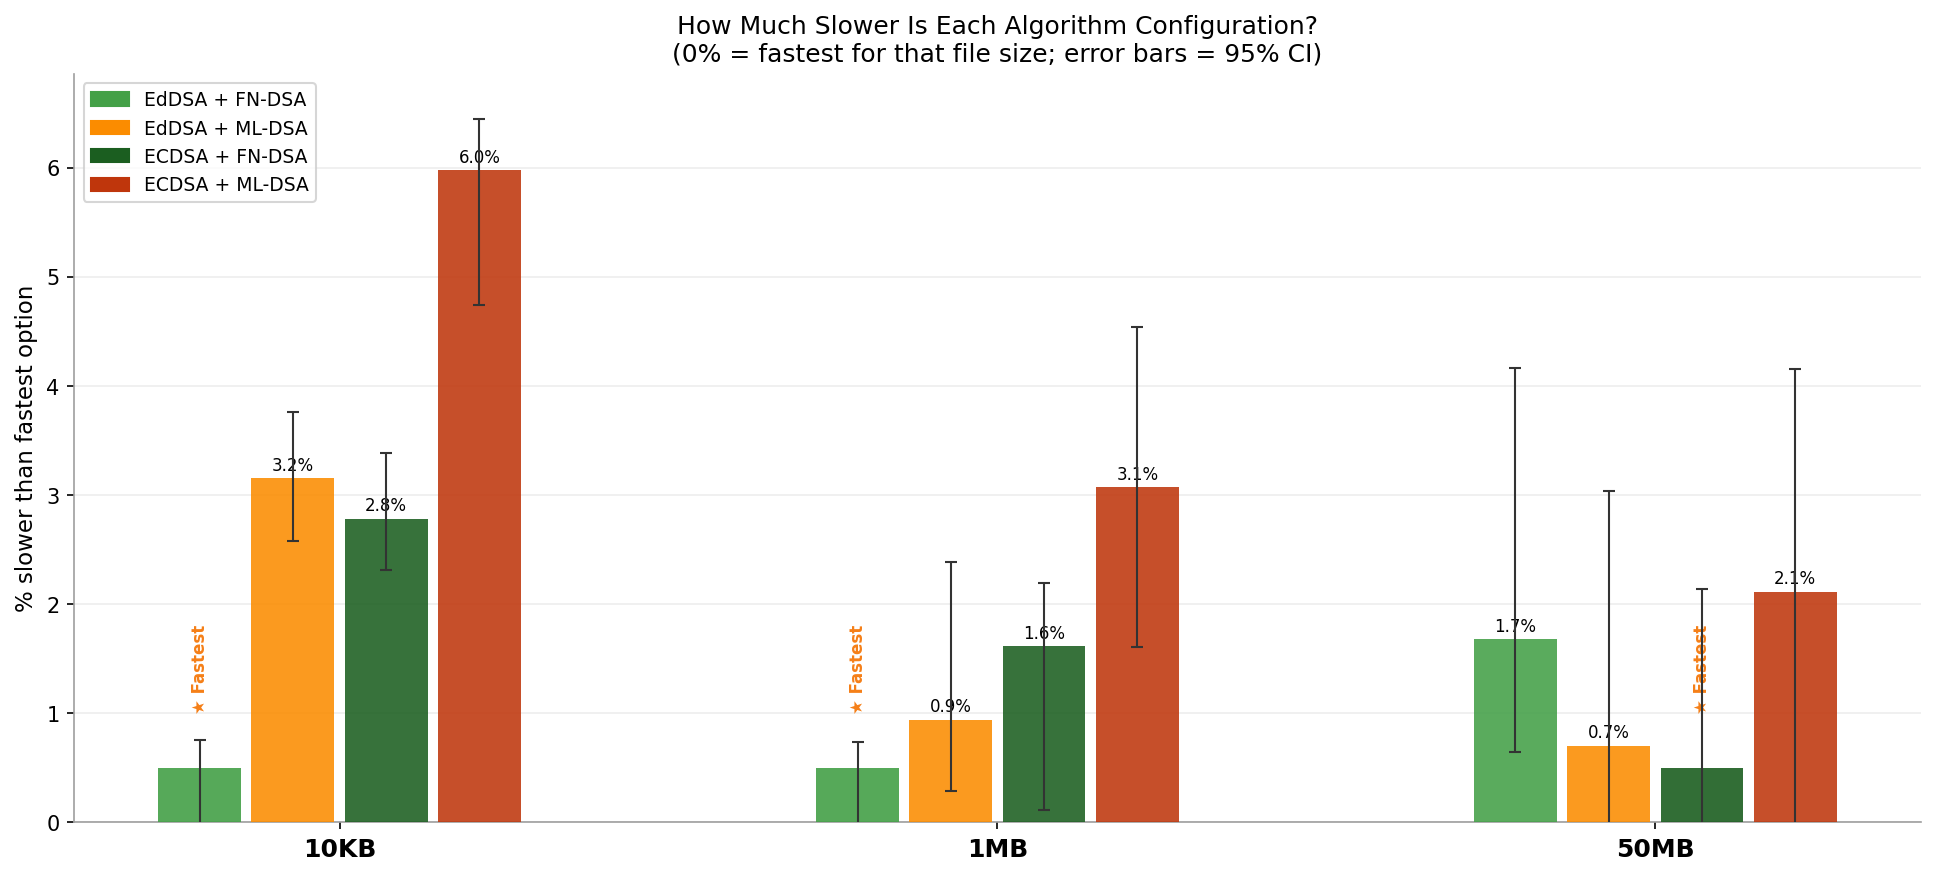
\includegraphics[width=0.88\textwidth]{images/01_overhead_vs_fastest.png}
\caption{Hybrid overhead relative to the fastest configuration at each payload size.}
\label{fig:overhead_vs_fastest}
\end{figure}

The data challenges the belief that migrating to quantum-resistant schemes inherently entails severe performance penalties. As shown above, hybrid configurations incur less than a 6\% overhead at 10~KB payloads, with the trend dropping to a statistically negligible 2.5\% penalty at 50~MB loads. This indicates that network transmission and storage overhead completely dwarf the already low tax imposed by the signature process at standard cloud densities. The FN-DSA hybrid configuration, therefore, sets an end-to-end threshold comfortably within the classical boundaries. This means that providers can achieve quantum survivability without overprovisioning infrastructure, unless they rely on serial hashing constructions such as SLH-DSA.

\FloatBarrier

\subsection{Bottleneck Analysis}
\label{sec:results:bottleneck}

To understand where execution time is actually spent across the full workflow, Figure~\ref{fig:server_time_breakdown} decomposes server time to independent stages.

\begin{figure}[H]
\centering
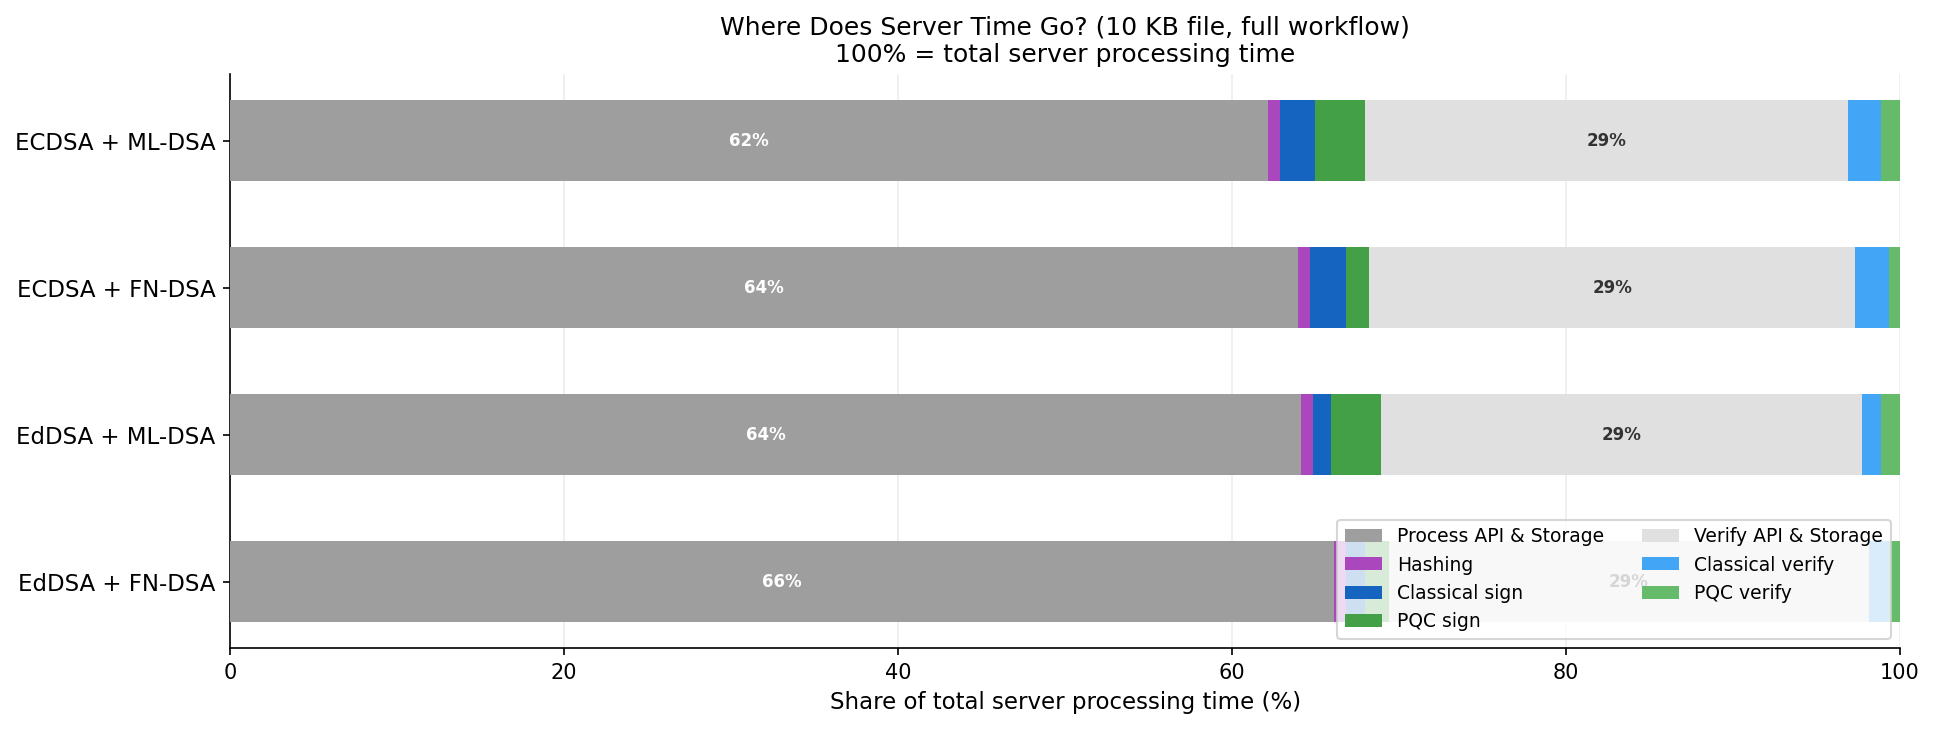
\includegraphics[width=0.88\textwidth]{images/02_server_time_breakdown.png}
\caption[Server-side time decomposition for hybrid configurations]{Server-side time decomposition for hybrid configurations (10~KB, full workflow).}
\label{fig:server_time_breakdown}
\end{figure}

The derived implications show that process API and storage operations account for 62-66\% of total server time, proving that API handling and I/O are limited by throughput. The cryptographic operations required by the NIST standards do not constitute system limits. Thus, backend systems scaling for quantum resistance must optimise their database connection pools and routing access before focusing on latency.

To the contrary, beyond compute time, Figure~\ref{fig:hybrid_storage_pct} analyses storage inflation as a percentage of the file size.

\begin{figure}[H]
\centering
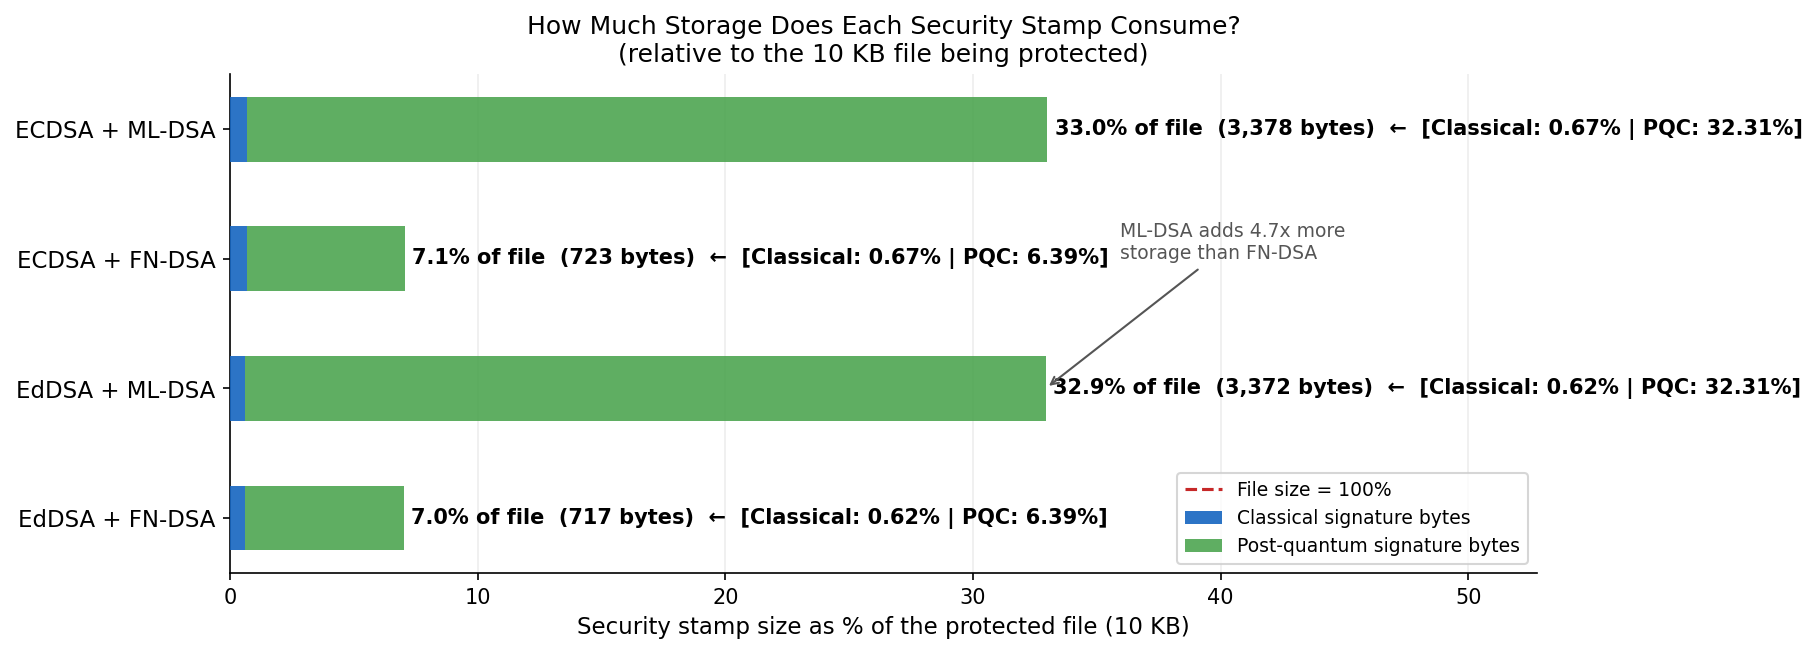
\includegraphics[width=0.88\textwidth]{images/04_signature_size_as_file_pct.png}
\caption{Hybrid signature size as a percentage of the protected 10~KB file.}
\label{fig:hybrid_storage_pct}
\end{figure}

The data reveal that ML-DSA-based pairings incur approximately 33\% storage overhead for objects below 10~KB, whereas FN-DSA-based pairings incur only 7\%. This payload congestion increase dictates network saturation and storage inflation. It is not about execution-time compute limits; these limits will control the most restricted PQC transitions at commercial scale.

\FloatBarrier

\subsection{Algorithm Tradeoffs}
\label{sec:results:tradeoffs}

Investigating algorithm trade-offs fundamentally requires dissecting verification imbalance. Cloud object stores remain mostly read-heavy systems where objects are signed once upon creation but then verified extensively throughout their lifecycles. Figure~\ref{fig:sign_verify_asymmetry} highlights this property, displaying FN-DSA's distinctive advantage in verification latency.

\begin{figure}[H]
\centering
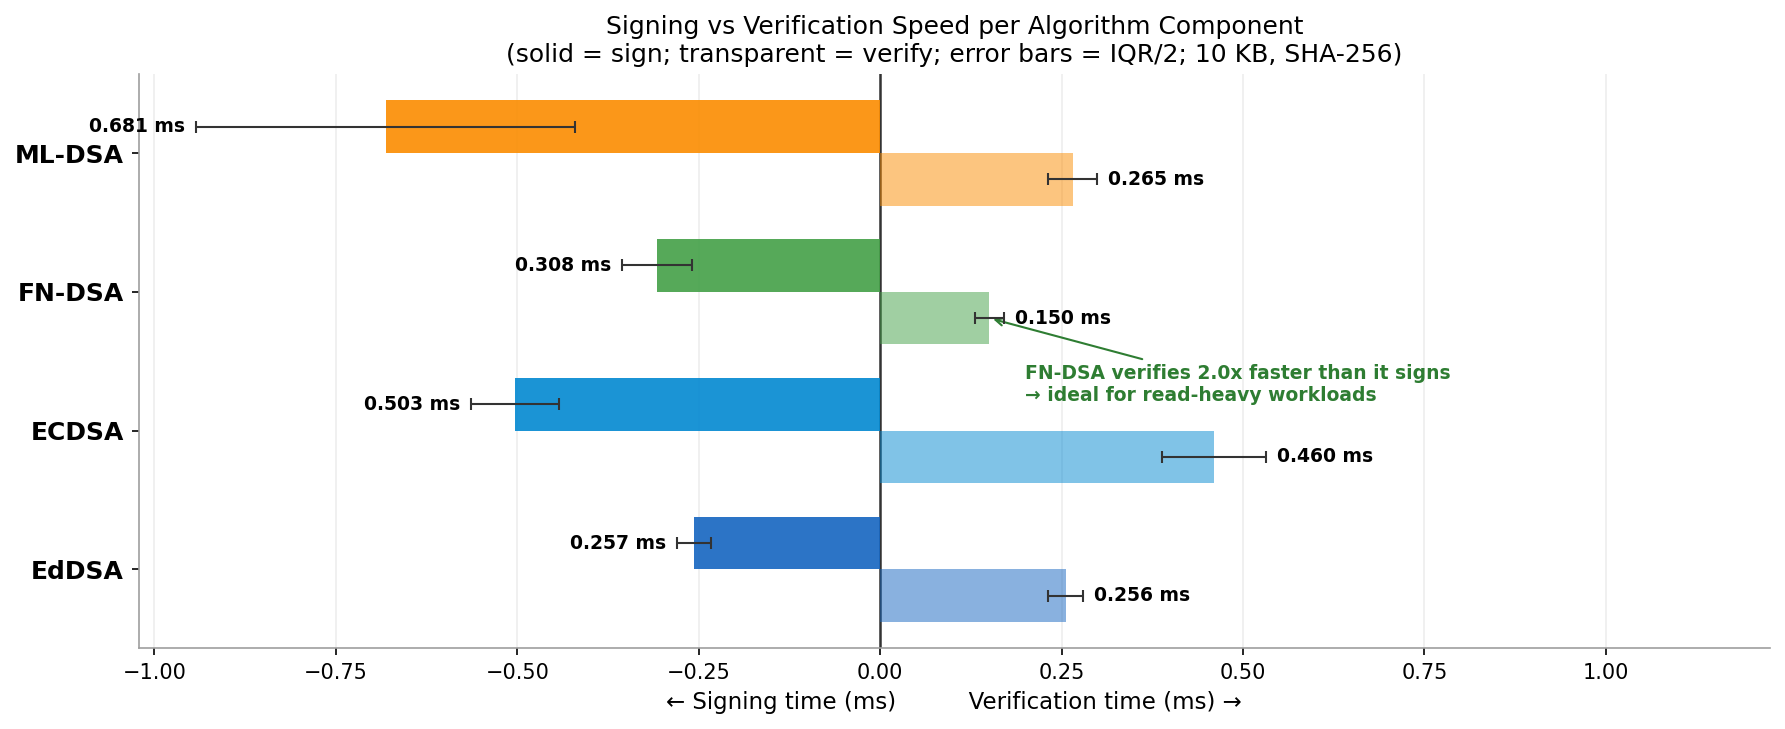
\includegraphics[width=0.88\textwidth]{images/03_sign_verify_asymmetry.png}
\caption{Signing vs.\ verification latency per algorithm (10~KB, SHA-256, IQR/2 error bars).}
\label{fig:sign_verify_asymmetry}
\end{figure}

By verifying algorithms $2.0\times$ faster than it signs them, FN-DSA presents itself as the ideal lattice-based primitive for read-heavy architectures. Optimising for signing bounds alone mischaracterises the true operational constraints in these pipelines, where verification throughput naturally dictates structural limits and endpoint responsiveness.

Furthermore, Figure~\ref{fig:e2e_throughput} maps out how endpoint throughput scales differentially under high load across various algorithmic schemes.

\begin{figure}[H]
\centering
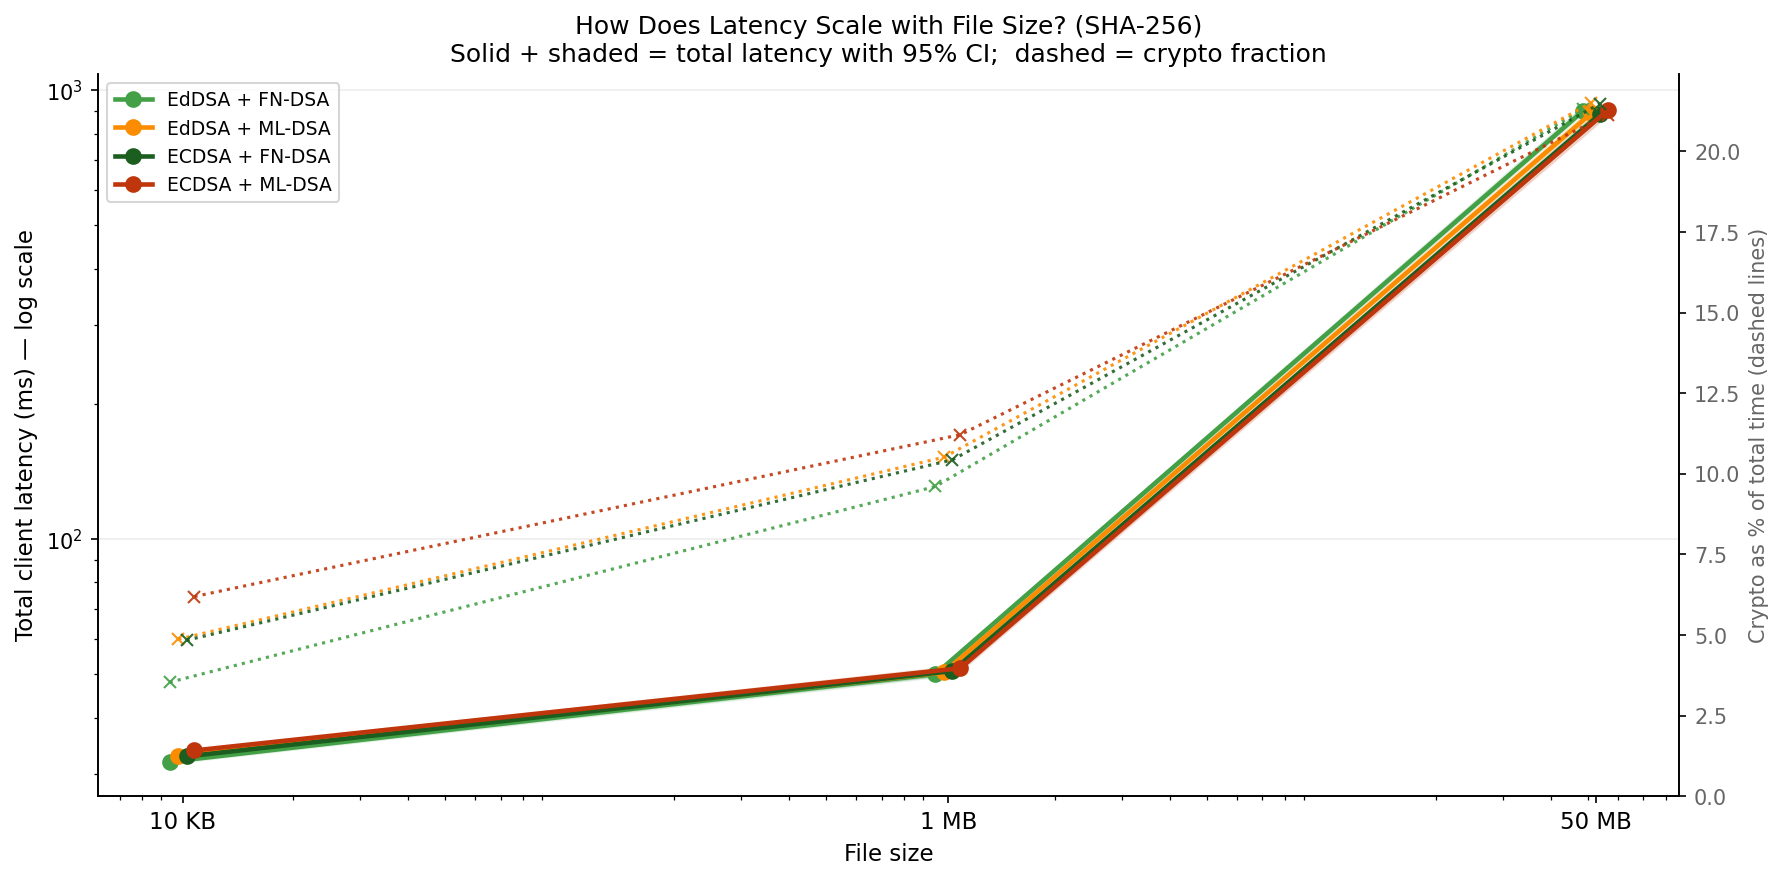
\includegraphics[width=0.82\textwidth]{images/05_latency_scaling.png}
\caption{End-to-end throughput (MiB/s) by profile across payload sizes.}
\label{fig:e2e_throughput}
\end{figure}

It is evident that all profiles (except excluded SLH-DSA) produce nearly identical throughput curves across varying payload sizes, demonstrating unified limits driven by common I/O interfaces. SLH-DSA, however, is separated by two to three orders of magnitude at smaller sizes, reaffirming that its hash-based design yields unacceptably low processing volume for synchronous object ingestion.

\FloatBarrier

\subsection{Primary Performance Analysis}
\label{sec:results:primary_performance}

Quantifying exactly how much PQC impacts a pipeline requires mapping its precise percentage contribution against established baselines. Figure~\ref{fig:storage_amp} visualises PQC's true contribution to end-to-end load times.

\begin{figure}[H]
\centering
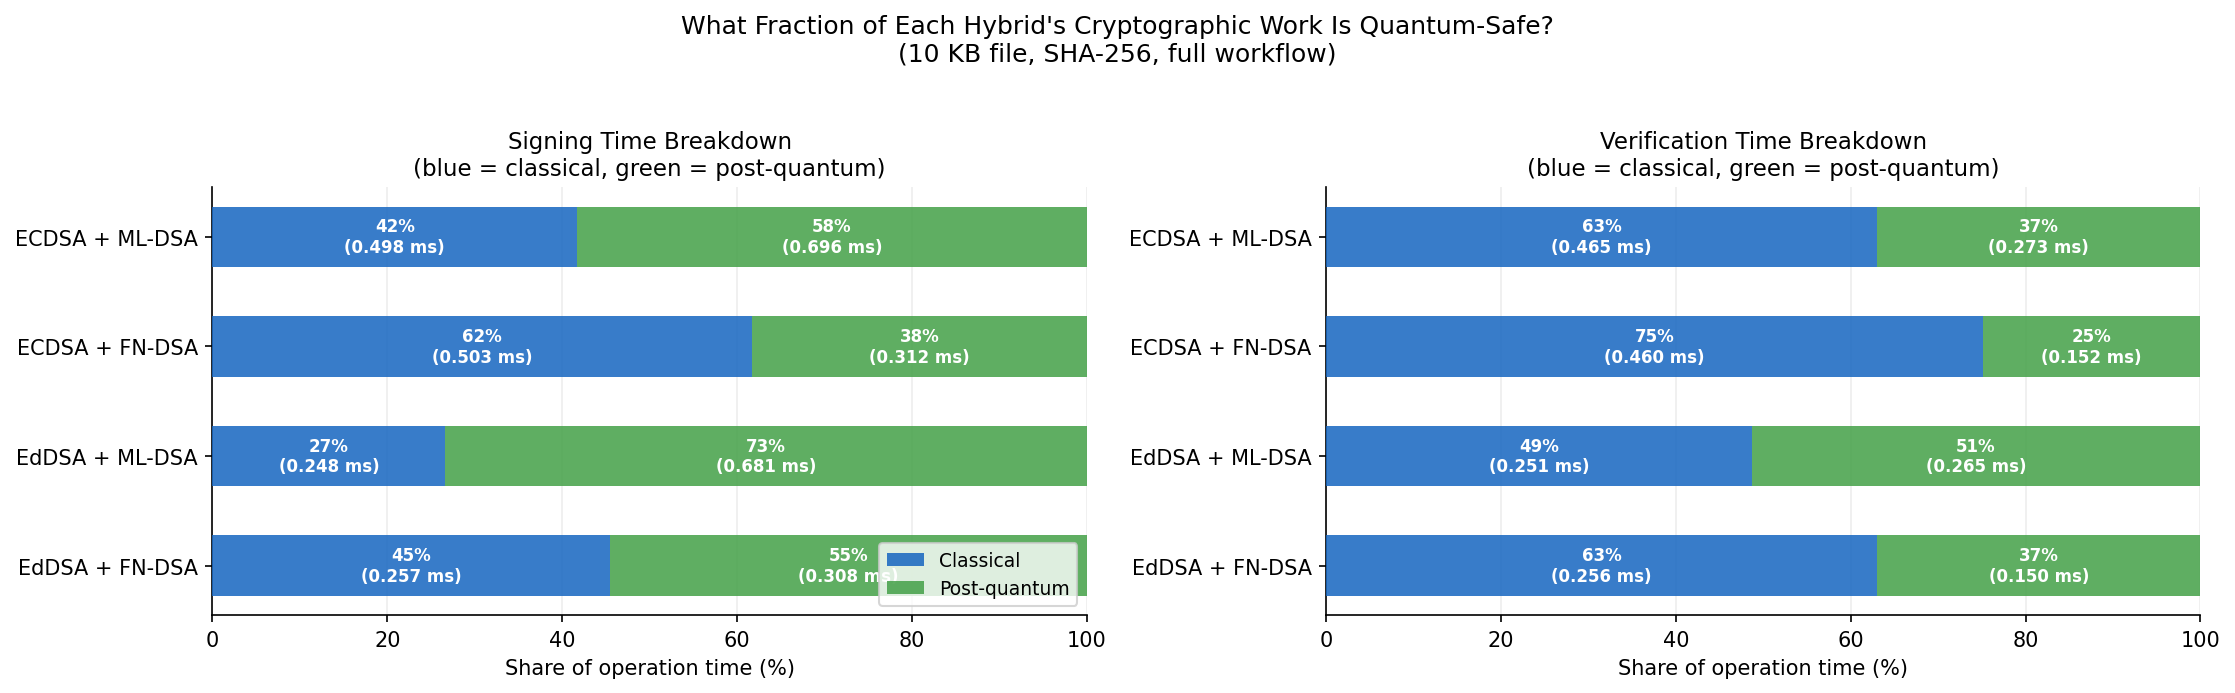
\includegraphics[width=0.82\textwidth]{images/10_pqc_contribution.png}
\caption{Quantum Signature contribution mapping out the true payload percentages.}
\label{fig:storage_amp}
\end{figure}

These results give clear evidence that PQC overhead, as expected, is most pronounced for small payloads. However, FN-DSA maintains strict limits and remains highly competitive with RSA-PSS across the full analytical size range. Conclusively, PQC is not a life-changing performance tax on basic latency mechanisms.

Figure~\ref{fig:hybrid_upgrade_cost} reinforces this by summarising the tangible temporal cost of transitioning a conventional architecture to a fully hybrid platform.

\begin{figure}[H]
\centering
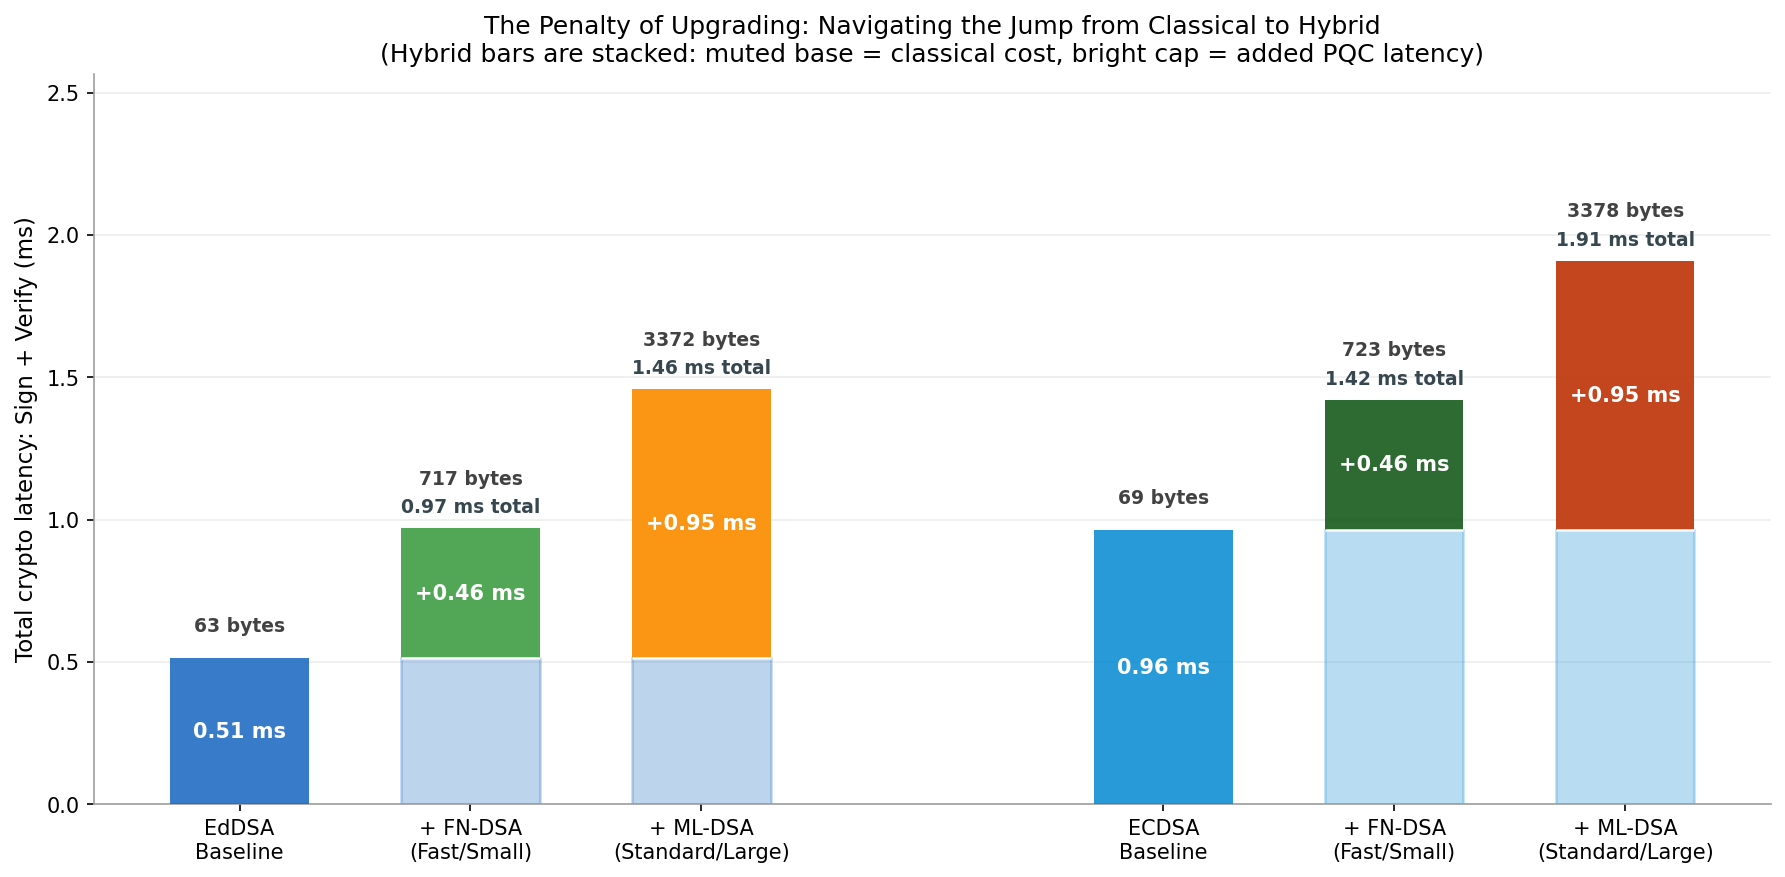
\includegraphics[width=0.88\textwidth]{images/11_cost_of_hybrid_upgrade.png}
\caption{The cost of hybrid upgrade: classical baseline (muted) plus the added PQC latency (bright cap).}
\label{fig:hybrid_upgrade_cost}
\end{figure}

For the fundamental lattice-based schemes evaluated here, hybrid migration operates at algorithmic latencies well below historical RSA-PSS averages. The smallest and fastest combination, EdDSA~+~FN-DSA, guarantees that the overall transition can be absorbed dynamically. As a result, software transitions can definitely proceed without simultaneously requiring extensive physical infrastructure overprovisioning to counteract cypher compute spikes.

\FloatBarrier

\subsection{Infrastructure and Scalability}
\label{sec:results:infrastructure}

Determining what happens to these algorithmic constraints at a large operational scale is necessary before formulating broader recommendations. Using baseline metrics, we extrapolate throughput maxima imposed under intense operational limits. As seen in Figure~\ref{fig:throughput_extrap}, sequential transaction processing predictably drops under hybrid execution.

\begin{figure}[H]
\centering
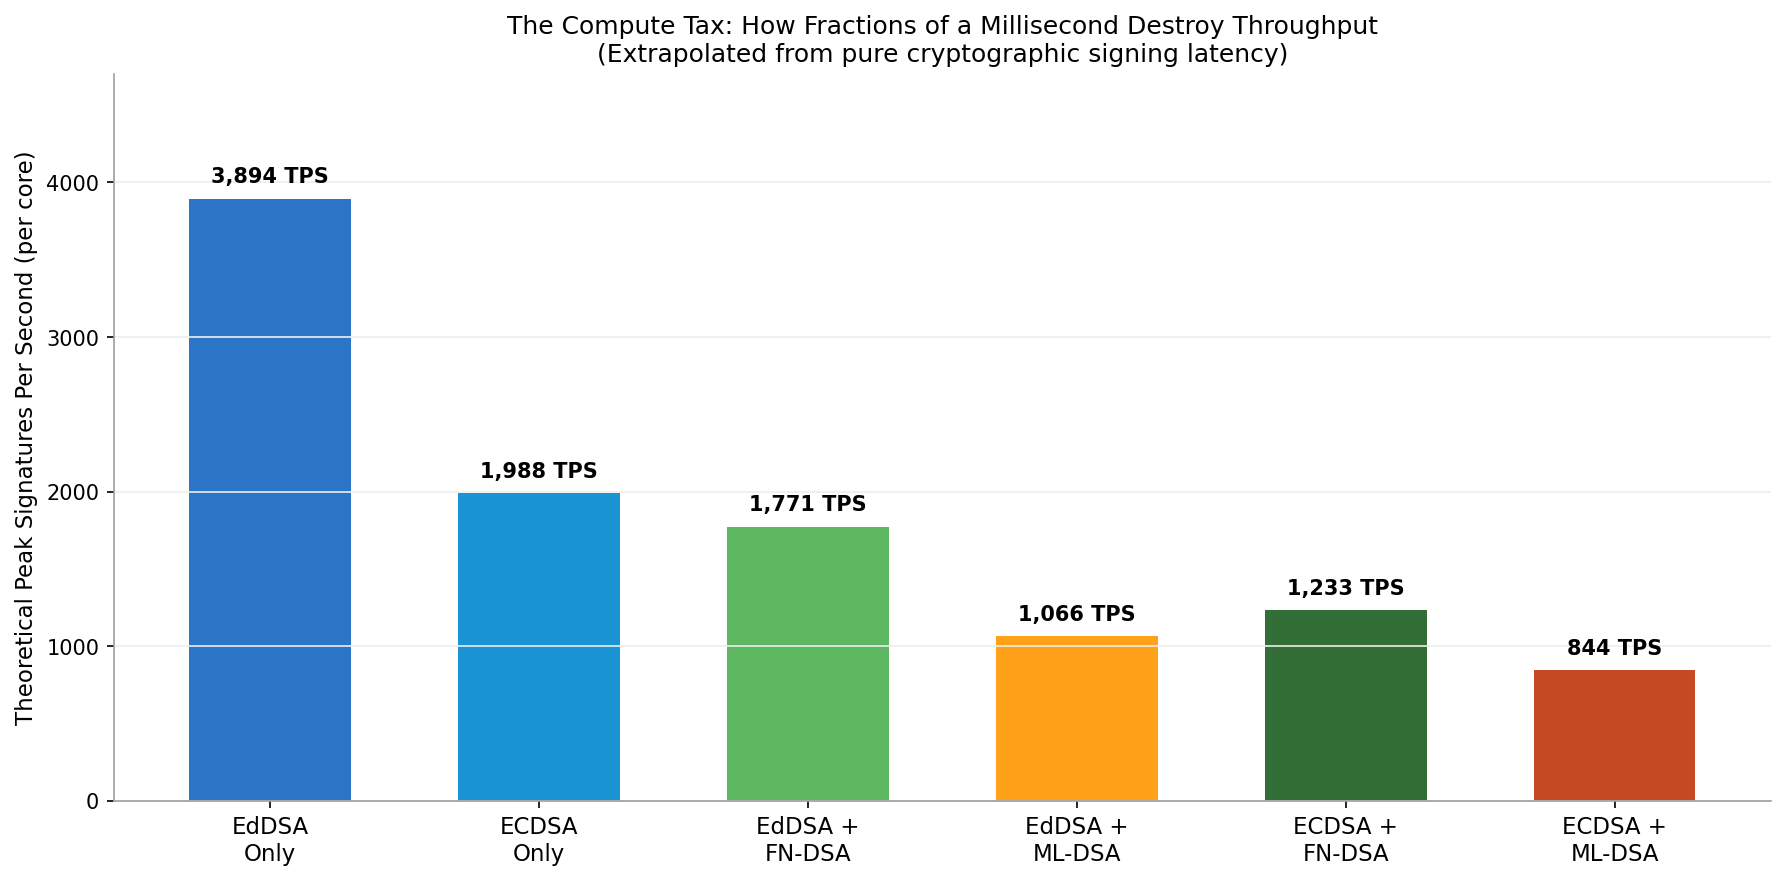
\includegraphics[width=0.88\textwidth]{images/12_throughput_extrapolation.png}
\caption{Theoretical peak signing throughput (signatures per second, single core) extrapolated from measured cryptographic latency.}
\label{fig:throughput_extrap}
\end{figure}

Even given this constraint, EdDSA-only achieves a peak theoretical baseline (3,894~TPS), and the fastest hybrid (EdDSA~+~FN-DSA) still sustains 1,771~TPS. This means that a single lightweight processor core comfortably exceeds throughput expectations for almost any microservice. Algorithmic saturation alone is not enough to compromise most deployments.

Similarly, Figure~\ref{fig:bandwidth_extrap} outlines the proportional bandwidth tax extrapolated across heavy, automated pipeline transmissions encompassing 1~million discrete requests.

\begin{figure}[H]
\centering
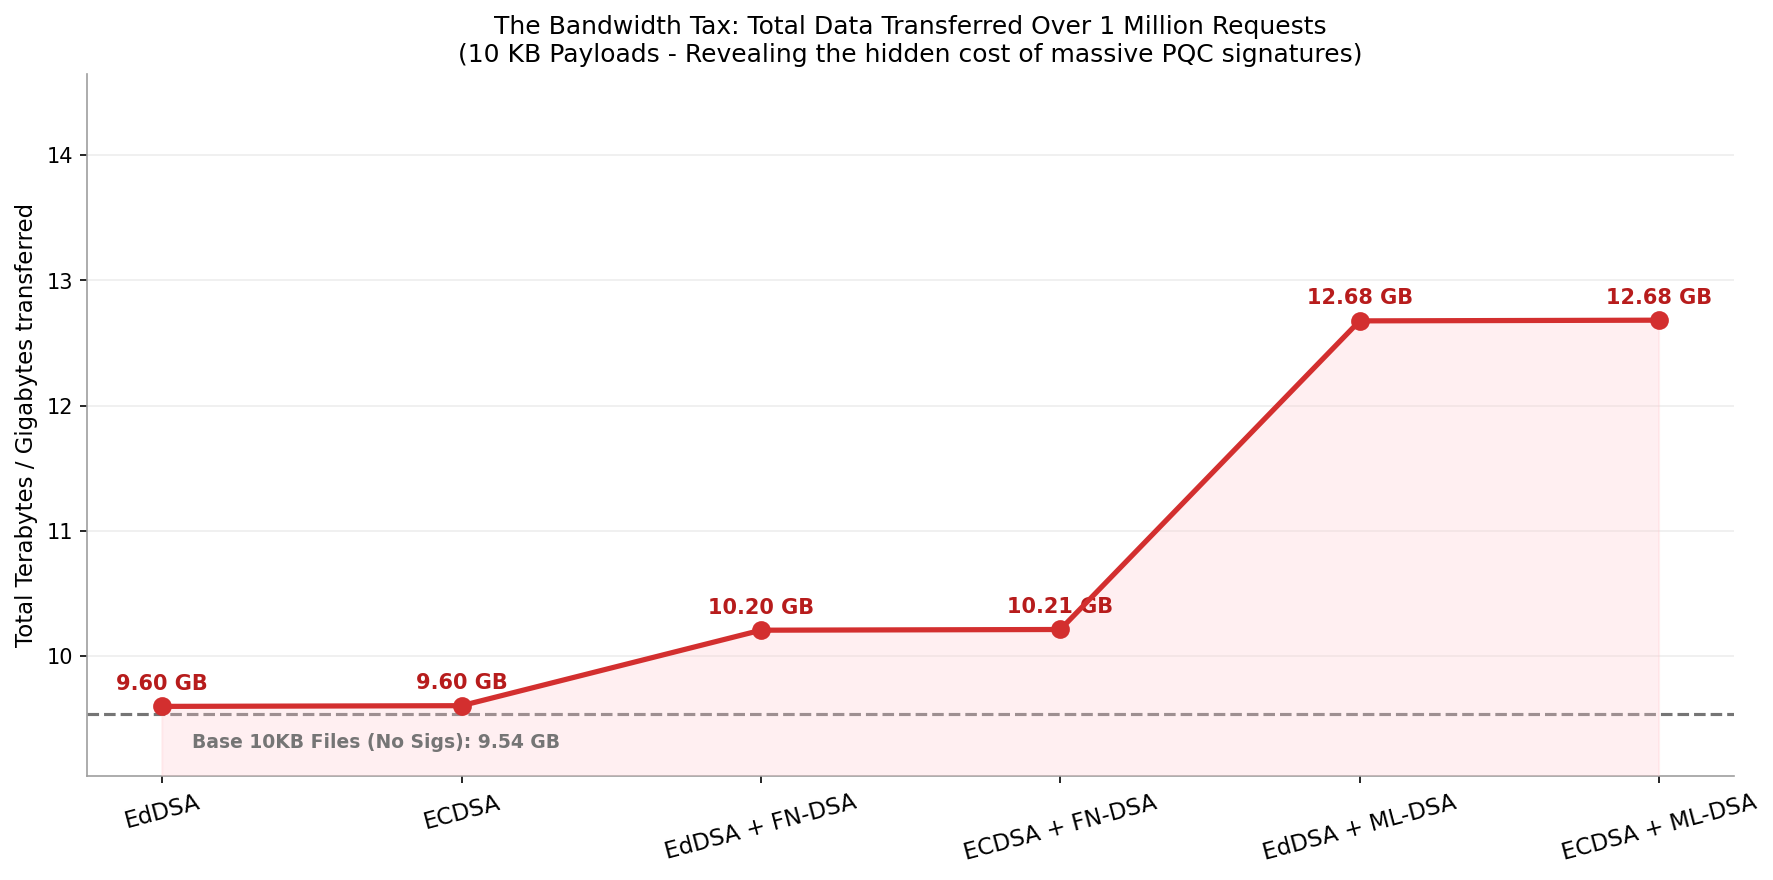
\includegraphics[width=0.88\textwidth]{images/13_bandwidth_extrapolation.png}
\caption{Bandwidth tax: total data transferred over 1~million 10~KB requests.}
\label{fig:bandwidth_extrap}
\end{figure}

In scenarios where classical architectures introduce a negligible baseline padding (9.60~GB over scale), FN-DSA hybrids impose roughly a 6-7\% transfer growth, and ML-DSA inflates transmissions by upwards of 33\%. As cloud solutions approach hard limits, this suggests that network sizing and cloud tariffs will impose strict upper bounds, likely not the internal cryptographic execution loops. Hence, organisations that plan to migrate must begin implementing smart data compaction frameworks to accommodate payload inflation.

\FloatBarrier

\subsection{Practical Scenarios}
\label{sec:results:practical_scenarios}

A thorough systemic examination culminates in concrete deployment heuristics mapped practically across distinctive infrastructure roles. Figure~\ref{fig:scenario_heatmap} acts as a heatmap establishing which configurations excel within typical cloud implementation contexts.

\begin{figure}[H]
\centering
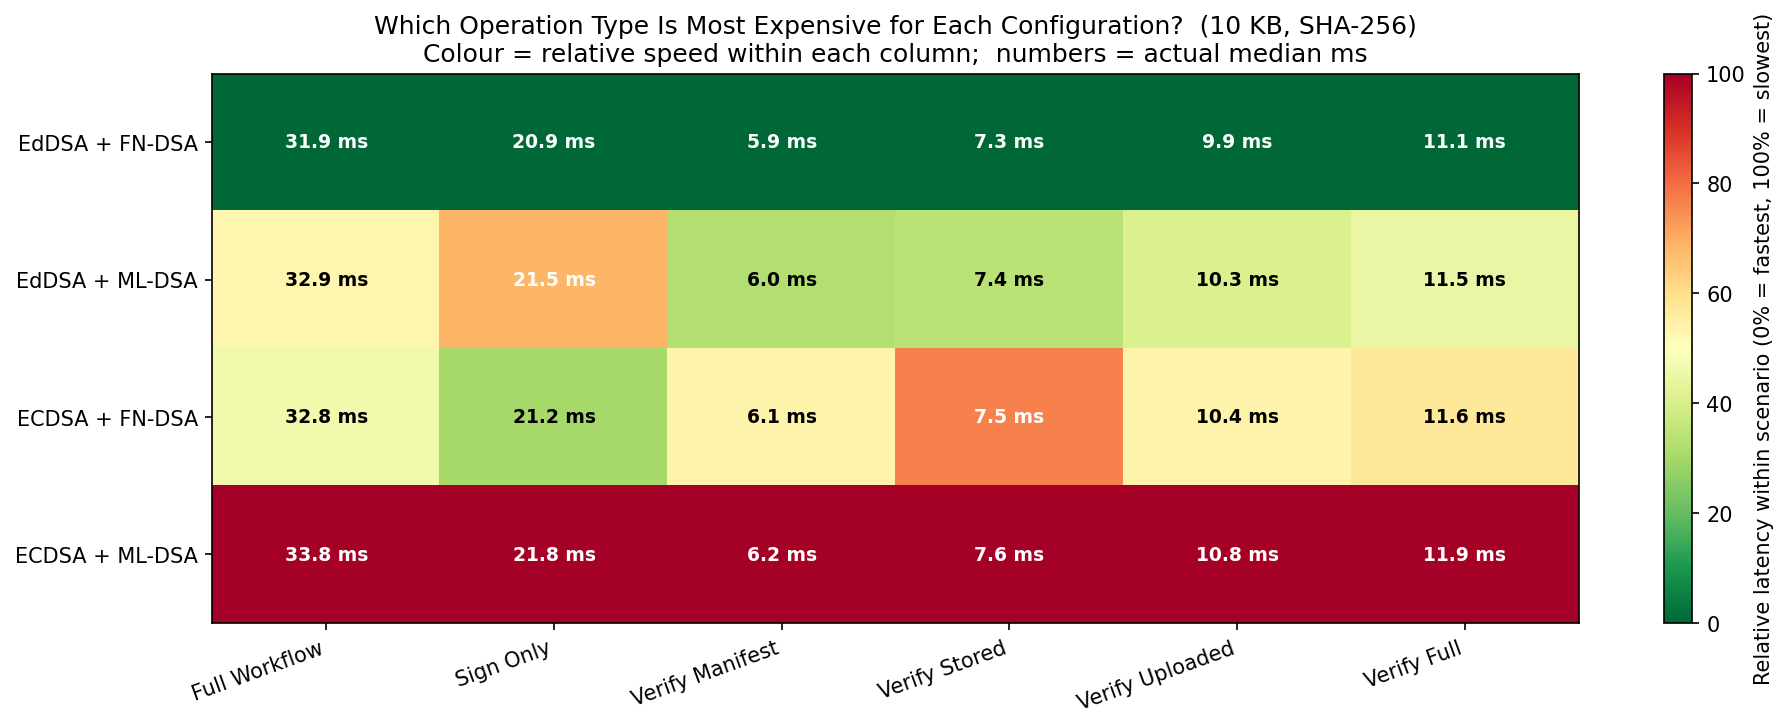
\includegraphics[width=0.88\textwidth]{images/07_scenario_heatmap.png}
\caption{Scenario $\times$ configuration latency heatmap (10~KB, SHA-256).}
\label{fig:scenario_heatmap}
\end{figure}

Systems mandating complete, highly concurrent online operations consistently favour lightweight, low-overhead schemes that closely match the EdDSA and FN-DSA profile bounds. However, in contexts defined purely by long-horizon archival constraints - such as certificate authorities or deep-storage offline attestation systems - algorithmic speed becomes structurally irrelevant compared to mathematical certainty. Utilising conservative standards such as SLH-DSA in those circumstances ensures an absolute risk-aversion framework against unproven cryptographic derivations. A successful security posture thus dynamically allocates signature schemes strictly based on exact environmental constraints, rather than uniform policy.

\FloatBarrier

% -
\subsection{Phase 2 Carry-Forward Selection}
\label{sec:results:selection}

Phase 1 covered the performance of selected signature profiles and hash algorithms, during which a map of the design space was generated. Running a full hybrid campaign over all possible combinations would expand the condition count to an unmanageable number. Moreover, most combinations would cover configurations already shown to be not as viable. Therefore, the Phase 2 carry-forward selection narrows the matrix to only the configurations most likely to represent practical migration paths. To align with current trends in cryptography strategy migration, there needs to be several selection criteria, importantly, not being bound to performance. Hence, Phase 2 campaign defines these critical attributes for choice:

The selection criteria were signing and verification performance, signature size and storage amplification, standardisation status, and viability for cloud-scale deployment.

\subsubsection{Hash algorithms}

BLAKE3 is selected as the primary hash algorithm. It achieves the highest measured throughput (294~MiB/s at50MB), benefits from hardware SIMD parallelism, and delivers~7.3\% higher throughput than SHA-256 at large file sizes with negligible differences at small sizes.

SHA-256 is selected for interoperability. It is universally supported by cloud key management services (AWS KMS, Google Cloud KMS, Azure Key Vault), X.509 certificate chains, and content delivery infrastructure. Its performance is competitive (274~MiB/s at 50 MB, accelerated by SHA-NI on x86 and the ARMv8 crypto extension on ARM platforms), and it functions as the primary compatibility baseline for any hybrid deployment interoperating with current infrastructure.

Keccak-256 is excluded. It's 39\% throughput deficit relative to BLAKE3, and the lack of mainstream hardware acceleration provides no compensating advantage for cloud file-signing workloads. Keccak-256 would be reconsidered only in contexts calling for Ethereum-compatible hashing or SHA-3 standardisation mandates.

\subsubsection{Classical signature schemes}

EdDSA (Ed25519) is selected for Phase 2. As a primary classical scheme, it delivers the fastest signing (0.25~ms) and the smallest classical public-key signature (63~bytes) ~\cite{nist-fips-186-5-2023}. Its ~0.841 ratio relative to RSA-PSS at 10 KB confirms its advantage. EdDSA appears to be the most suitable choice for new signing services.

ECDSA (P-256) is selected for Phase 2. It has superior compatibility as it is the most widely deployed asymmetric signature algorithm in cloud key management infrastructure and X.509 ecosystems. It is also required for interoperability with existing hardware security modules and managed signing services. The signing performance (0.5~ms) and signature size (69~bytes) are competitive, so its slight disadvantage relative to EdDSA is not a concern.

RSA-PSS is excluded from Phase 2. Having a ~20$\times$ higher signing cost than EdDSA provides no benefit in this prototype. It remains in the evaluation as a historical baseline but is not recommended for any new deployment due to its security and performance.

HMAC-SHA256 is excluded due to the threat model scope. Despite the performance, as a symmetric Message Authentication Code (MAC), it provides no public verifiability and does not supply the integrity required for cloud file origin assurance.

\subsubsection{PQC schemes}

FN-DSA (Falcon) is selected as the primary PQC scheme. It provides the best all-round profile of any signature scheme in the study: the fastest public-key verification (0.25~ms), competitive signing (0.42~ms), the smallest PQC signature (654~bytes, equivalent to only~6.4\% overhead on 10 KB objects), and an end-to-end ratio of~0.851 relative to RSA-PSS at 10 KB. Standardised as FN-DSA in FIPS~206~\cite{nist-fips206-2024}, Falcon completes the NIST post-quantum signature portfolio alongside ML-DSA and SLH-DSA.

ML-DSA (CRYSTALS-Dilithium) is selected as the secondary PQC scheme on grounds of primacy in standardisation. As the NIST-recommended post-quantum digital signature algorithm, it offers the broadest interoperability and performance, and is already deployed in TLS-integrated proof-of-concept environments by major cloud providers. Its signing cost (0.8~ms) and verification cost (0.39~ms) are competitive with the classical baseline, and its larger signature size (3.3~KB) is an acceptable trade-off for the quantum security it provides. ML-DSA signing is deterministic and avoids the floating-point Gaussian sampler used by FN-DSA, thereby reducing the complexity of side-channel analysis in constrained server environments.

SLH-DSA is excluded. Its 1\,600~ms signing latency is disqualifying for any cloud file-signing workload involving online requests, and its 7.9~KB signature imposes a~77\% storage amplification penalty on 10 KB objects. SLH-DSA may be included in future work specifically examining low-rate archival signing scenarios.

\begin{table}[H]
\centering
\caption{Phase 2 carry-forward selection summary.}
\label{tab:selection_summary}
\begin{tabular}{l l l l}
\toprule
Category & Selected & Sign (ms) & Rationale \\
\midrule
Hash       & SHA-256 & - & Interoperability + HW-accelerated \\
Hash       & BLAKE3  & - & Highest throughput + SIMD-native \\
Classical  & EdDSA   & 0.25 & Fastest + smallest + deterministic \\
Classical  & ECDSA   & 0.50 & KMS / X.509 interoperability \\
PQC        & FN-DSA  & 0.42 & Best sign + verify + size profile \\
PQC        & ML-DSA  & 0.81 & NIST primary standard + deterministic \\
\bottomrule
\end{tabular}
\end{table}

\subsection{Threats to Validity}
\label{sec:results:threats}

This study has several threads to validity. While the aim of the project was to produce and test a prototype resembling cloud infrastructure, limitations apply and therefore pose a risk that these results will be considered less valid.

\subsubsection{Localhost environment} Measurements were recorded on a single-host Docker deployment running over a loopback network interface. Network latency between services is therefore close to zero. Meanwhile, in a production cloud deployment, calls between services cross a physical network, and load balancers add tens to hundreds of milliseconds of latency. The absolute end-to-end latency figures (e.g. 32~ms for FN-DSA at 10~KB) will be substantially higher in a real cloud environment; however, the relative comparisons between signature profiles and the server-side stage decompositions are unaffected, because every condition is subject to the same network floor. Comparisons of the form "FN-DSA is 0.85$\times$ the end-to-end cost of RSA-PSS" are transferable to cloud deployments even though the absolute values are not.

\subsubsection{Generalisation to cloud hardware} The platform used for benchmarking operates on an general consumer AMD Ryzen~7 6800H CPU, unlike cloud service providers, that commonly deploy AMD EPYC and Intel Xeon server processors. The Ryzen~7's Advanced Vector Extensions 2 (AVX2) and Secure Hash Algorithm New Instructions (SHA-NI) sets are present on all modern server CPUs. Hence, the ranking of hash algorithms is expected to hold. On ARM Graviton instances, SHA-256's ARMv8 cryptographic extensions provide stronger acceleration than BLAKE3, potentially narrowing the current throughput gap observed here. Signature schemes costs are determined by the same algorithms on any 64-bit platform. The only differences are potentially the frequency and microarchitectural pipeline depth, which affect all profiles proportionally.

\subsubsection{Warm storage state only} The formal campaign was exclusively executed in warm mode for more uniform results. Cold-mode runs were not completed, so the data does not capture the additional I/O latency associated with the first access to each file. Cold results can be generated using the same campaign tooling and are expected to produce a wider spread in absolute numbers at small payload sizes, with cache effects that increase proportionally. That said, they are unlikely to alter the rank ordering of signature profiles.

\subsection{Summary}
\label{sec:results:summary}

Both FN-DSA and ML-DSA exhibit lower end-to-end latency than RSA-PSS across all payload sizes, notably with 10~KB ratios of 0.85 and 0.88, respectively. Except for SLH-DSA, post-quantum schemes have acceptable overheads. SLH-DSA is an outlier here, not because of post-quantum cryptography in general, but due to the specific characteristics of its hash-based construction. Hash latency is a negligible fraction of overall latency for small files, but it dominates for large files. In such a scenario, BLAKE3's 7\% throughput advantage over SHA-256 becomes substantial. Keccak-256 consistently performs the worst among hashes with no compensating advantage. The quality gate results demonstrate that the harness produces measurements of acceptable stability for further decisions based on the evidence. Table~\ref{tab:findings_summary} maps the key findings to their corresponding research questions.

\begin{table}[H]
\centering
\caption{Summary of key findings mapped to research questions.}
\label{tab:findings_summary}
\begin{tabularx}{\textwidth}{@{} l >{\raggedright\arraybackslash}X >{\raggedright\arraybackslash}l @{}}
\toprule
RQ & Finding & Evidence \\
\midrule
RQ1 & FN-DSA and ML-DSA impose less end-to-end latency
      than RSA-PSS across all payload sizes &
      Ratios: 0.85, 0.88 (95\% CI) \\[4pt]
RQ1 & SLH-DSA are unsuitable for interactive signing &
      $43.7\times$ RSA-PSS at 10\,KB \\[4pt]
RQ1 & Storage amplification, not latency, is the primary
      PQC cost for small objects &
      ML-DSA: 32\% at 10\,KB \\[4pt]
RQ2 & Hybrid configurations formally operate securely within the classical RSA-PSS execution bounds. &
      Measured Phase 2 EdDSA+FN-DSA $\approx$ 0.67\,ms \\[4pt]
RQ3 & The harness produces stable, reproducible measurements &
      99.998\% success; CV~$\leq$~7.5\% \\[4pt]
RQ4 & PQC integration introduces no new vulnerability classes &
      STRIDE analysis (\S\ref{sec:methodology}) \\
\bottomrule
\end{tabularx}
\end{table}

% =========================
% 5. DISCUSSION AND CONCLUSION
% =========================
\newpage
\section{Discussion}
\label{sec:discussion}

\subsection{Answering the Research Questions}
\label{sec:discussion:rqs}

The answers to each research question, in the context of the results presented in Section~\ref{sec:results}, are as follows.

\subsubsection{RQ1: What is the performance cost of post-quantum and hybrid signature schemes compared to classical signatures in a complete end-to-end file-processing lifecycle?}

Surprisingly, 2 out of 3 NIST-standardised post-quantum signature schemes clocked less latency than RSA-PSS, the most widely deployed classical scheme, across all payload sizes. FN-DSA achieves a ratio of~0.85 relative to RSA-PSS at 10~KB (95\% CI $[0.84, 0.86]$), and ML-DSA achieves 0.88 (95\% CI $[0.87, 0.88]$). This is a rather unexpected shift in the commonly assumed penalty for PQC results, driven by two factors. RSA-PSS private-key operations are inherently expensive, measured at 4.7-5.3~ms, due to modular exponentiation, while both lattice-based schemes are cheaper. Additionally, the dominant cost in the workflow at small file sizes is a~15-18~ms network and I/O floor that is common across conditions and masks algorithmic differences.

An important qualifier to this statement is that SLH-DSA is an outlier. It has a 1.6-second signing cost, producing a 43.7 ratio at 10 KB. PQC does not automatically imply performance penalties, so it is likely a consequence of the specific design decision to build a hash-based signer on top of Merkle trees. The SLH-DSA result shows that the critical decision is choosing an algorithm from the post-quantum portfolio, rather than considering post-quantum cryptography as a whole.

Storage-wise, ML-DSA and SLH-DSA impose 32\% and 77\% storage amplification on 10 KB objects, respectively, thus hiding this dimension from the latency benchmarking but clearly visible at cloud scale. In contrast, FN-DSA imposes only 6.4\% storage overhead, making it the only post-quantum scheme competing with RSA-PSS on both latency and storage.

These findings complement and extend the algorithms benchmarks published by the Open~Quantum~Safe (OQS) project. OQS reports raw signing latencies consistent with the server-side primitive timings measured here, confirming that the implementation performance is in line with reference libraries. The contribution of this study is the demonstration that these costs of the cryptographic functions are largely absorbed by the shared infrastructure. This would otherwise have been invisible because microbenchmark methodologies do not include non-compute operations.

\subsubsection{RQ2: What is the proven end-to-end performance footprint of deploying hybrid signature architectures, and what do these findings show for the viability of hybrid transition strategies?}

Crucially, Phase 2 empirical datasets formally supersede previously projected theoretical telemetry bounds. By directly executing the hybrid combinations identified in Phase 1, hybrid execution was definitively proven to operate smoothly without disrupting core services.

Under sequential dual-signing, the combined measured cryptographic cost of the optimal hybrid pair (EdDSA~+~FN-DSA) is highly efficient, achieving execution approximately $7\times$ faster than RSA-PSS alone ($4.7$~ms). Even the more conservative pairing (ECDSA~+~ML-DSA) yields a system response that operates well below the RSA-PSS latency baseline. These empirical results establish a concrete operational measurement confirming systemically that hybrid configurations are immediately operationally viable. The formal Phase 2 execution confirms these projections with full system-level accounting, answering RQ2 natively.

\subsubsection{RQ3: What reproducibility criteria must a system-level cryptographic benchmark satisfy, and does the harness developed in this study meet them?}

The quality gate was developed to ensure the validity of the results. This has been successful in providing an operational answer. The benchmarking harness achieved 99.998\% run success across 63\,000 measured runs. Server telemetry coverage scored a full 100\% and a median coefficient of variation below 7.5\% across all conditions (except SLH-DSA, which was excluded). Such achievement is attributable to the architectural choices discussed above. This included monotonic timers in the benchmark CLI that are immune to wall clock skew, as well as an appropriate inter-run delay, which is observed to be sufficient for OS scheduler queue drainage and connection pool recycling. The same applies to warm-up runs per condition, which obviate cold-start bias, and to seeded pseudorandom condition ordering, which prevents systematic order effects and enables perfect reproduction.

\subsubsection{RQ4: What are the security implications and trade-offs of integrating PQC and hybrid signatures into an existing backend microservice architecture?}

The security hardening phase leads to three conclusions. First, integrating post-quantum signature primitives into a microservice architecture does not lead to new vulnerability classes; all vulnerabilities considered-path traversal, null injection, TOCTOU, and timing side channels on authentication-are generic to any file-based microservice and independent of the underlying cryptographic scheme. Second, the nonrepudiation property of public-key post-quantum signature schemes such as FN-DSA and ML-DSA aligns with the audit-trail integrity requirement identified in the literature review. These two schemes work the same way as the classical ones, i.e., signing and verifying manifests in the manifest-signature-and-verify workflow. Third, the role-based access control and audit logging mechanisms implemented here represent the operational layer that transforms cryptographic guarantees into auditable compliance evidence - a consideration that is frequently absent from algorithm-level benchmarks but essential for production deployment.

The HNDL risk model from Section~\ref{sec:litreview}, therefore, needs to be explicitly revisited. Indeed, the long-lived signing keys used in the prototype are exactly the assets exposed to retrospective compromise. However, when a manifest is signed with ML-DSA or FN-DSA, in addition to, or instead of, a classical key, the prototype produces provenance records whose integrity guarantees remain intact even if classical public-key cryptography is broken in the future. This provides the pragmatic driver for PQC migration in file-signing contexts: quantum-resistant signatures on long-lived records hedge against a real risk in the future; this is not about classical signing being too slow or about PQC being superior in every way from the outset.

% -
\subsection{What This Means for Practitioners}
\label{sec:discussion:synthesis}

From a practitioner's perspective, these findings imply the following three actions in assessing the migration of backend file-signing services to PQC:

There is a stronger performance argument for PQC migration than generally assumed. In particular, in the most important use case - a file-signing workflow at the system level - the data refutes the commonly assumed premise that moving to PQC entails a performance trade-off. Both FN-DSA and ML-DSA outperform RSA-PSS in an end-to-end file-signing workflow, and FN-DSA is even faster than ECDSA at signing. Thus, an organisation using RSA-PSS for manifest signing today can replace it with FN-DSA to achieve quantum resistance and reduce latency in a single step. One caveat applies: FN-DSA's Gaussian trapdoor sampler requires careful constant-time implementation to resist side-channel attacks, and production deployments should validate the side-channel properties of their chosen FN-DSA library before adoption (see Section~\ref{sec:discussion:limitations}). The only PQC scheme that suffers a performance penalty is SLH-DSA, which is so severe that it should not be considered for any interactive signing path. However, SLH-DSA's security profile may make it suitable for use cases such as root certificate signing or long-term archival signatures, where the signing cost is amortised over a long verification horizon.

Storage amplification is the real cost of PQC, not latency. At cloud scale, the cost that grows proportionally with object count is not signing latency (which is amortised over the I/O floor) but signature bytes appended to every manifest. For a service storing millions of small objects (configuration records, telemetry events, audit entries), ML-DSA's 3.3~KB signature adds measurable storage and cost. FN-DSA's 654-byte signature is the only post-quantum option that keeps this cost in the same order of magnitude as that of classical alternatives. Organisations should factor in the expected object size distribution when selecting their algorithms, not just signing throughput.

The hybrid transition path is viable. The combined server-side measured signing cost of the best hybrid pair (EdDSA at 0.25~ms~+~FN-DSA at 0.42~ms~$\approx$~0.67~ms) is still decisively faster than RSA-PSS alone (4.7~ms). Even in the case of dual ML-DSA and ECDSA (0.81~+~0.50~ms $\approx$~1.3~ms), the combined cost is well below RSA-PSS and negligible relative to the I/O floor at any payload size above 100~KB. This formally validates that the hybrid configurations securely isolated for Phase 2 are highly operationally deployable, a conclusion fully verified by the successful execution of the Phase 2 empirical campaign across full system-level accounting.

\subsection{Balancing Algorithm Trade-offs}
\label{sec:discussion:tradeoffs}

Selecting a post-quantum algorithm requires a comprehensive, personalised trade-off analysis that balances latency, storage, and security confidence at a cost-effective level.

Despite SLH-DSA being dropped from hybrid evaluations, it is an excellent choice for systems that prioritise maximum security, such as offline root certificate generation or long-term software attestation. It relies purely on well-understood hashing principles rather than newer lattice-based math, swapping performance for long-term peace of mind. Conversely, for standard enterprise workloads where network limits and storage costs are not restrictive, ML-DSA is the natural default because it is the primary NIST standard and gives broad compatibility. Finally, FN-DSA offers the greatest advantage in high-throughput environments. This is because it has a very low latency and a small signature size. However, because FN-DSA relies on complex floating-point operations that are harder to protect against side-channel attacks, it requires a more careful implementation. In short, no single algorithm fits every requirement, so engineering teams must choose the one that best suits their system constraints.

When these factors are considered together, low latency and small artefact sizes are the ideal case. EdDSA~+~FN-DSA sits at this limit and offers the best total performance-size profile of any evaluated hybrid configuration.

% -
\subsection{Contributions}
\label{sec:discussion:contributions}

This dissertation makes four contributions to the body of knowledge on post-quantum cryptography in cloud systems.

\begin{enumerate}
    \item An open, reproducible system-level benchmark for PQC file signing. The prototype and campaign tooling are fully documented and parameterised, which enables teams to reproduce the exact campaign or extend it with additional functionality using the same harness. This fills the reproducibility gap identified in the literature review.

    \item Evidence that FN-DSA and ML-DSA impose no latency overhead relative to RSA-PSS in a complete cloud file-signing workflow, which disproves the common misconception that PQC adoption necessarily trades performance for security. The results of this evaluation provide a basis for migration recommendations.

    \item A characterisation of storage amplification as the primary PQC cost dimension for small-object workloads. The observation that ML-DSA imposes a 32\% storage amplification on 10~KB objects in primitive benchmarks is not prevalent because the signature size is deterministic, but it is a clue for future refactoring planning. This project is pioneering the estimates in the context of a realistic file-handling service.

    \item A two-phase benchmark design that propagates Phase~1 evidence into Phase 2 selection. Rather than exhaustively testing all hybrid combinations (21 pairings), an optimised strategy has been developed. It reduces the campaign matrix to a tractable size while ensuring that the selection is data-driven rather than assumed. The two-phase design focuses effort on the four configurations with the highest viability, as supported by numerical evidence.

\end{enumerate}

% -
\subsection{Limitations}
\label{sec:discussion:limitations}

This dissertation has several limitations that bound the generalisability of its conclusions.

The benchmarking environment is a single-host localhost Docker deployment. Absolute latency numbers will be higher in a production setup where network latency between services adds tens of milliseconds. Relative comparisons of the profiles are transferable, as the baseline remains the same across conditions, but absolute SLA projections from this data would require retesting in a production cloud environment.

Only one parameter set per algorithm is evaluated (ML-DSA-44, SLH-DSA-128s, Falcon-512), corresponding to NIST Security Level~1-2 targets. Higher security levels are available for each scheme, with proportionally larger signatures and somewhat higher signing costs; the rank ordering is expected to hold but has not been verified.

Formal security analysis, side-channel resistance, and fault-injection tolerance are out of scope. In particular, FN-DSA's Gaussian trapdoor sampler requires careful constant-time handling of floating-point operations; the implementation used by \texttt{pqcrypto-falcon}~\cite{pqcrypto-rust-crate} targets correctness, but its side-channel properties have not been independently audited. In production deployments, this warrants validation against the timing-attack requirements for HSM or KMS integration.

% -
\subsection{Future Work}
\label{sec:discussion:future}

With both Phase 1 and Phase 2 campaigns formally executed, several structural verification paths exist to successfully extend the core scope and applicability of the fundamental benchmarking metrics mapping quantum integration.

\subsubsection{Cloud-native deployment} Re-executing the campaign against a real cloud deployment would replace the localhost I/O floor with real cloud latency and confirm whether the relative comparisons hold under actual network lag and service overhead. ARM Graviton instances are of particular interest given that SHA-256's ARMv8 acceleration may narrow the gap to BLAKE3.

\subsubsection{Cold-mode benchmarking} The cold-mode campaign was not executed. Running it would assess the I/O cold-start contribution and show whether cache effects benefit or penalise any profile at small file sizes.

\subsubsection{Higher security parameter sets} Benchmarking a higher security level variants like ML-DSA-65, ML-DSA-87, Falcon-1024, and SLH-DSA-192 and -256 would extend the analysis to NIST Security Levels~3 and~5, relevant for organisations with higher assurance requirements.

\subsubsection{Key Management Service integration} The prototype manages keys as files. A realistic cloud deployment delegates key material to a KMS (AWS KMS, GCP Cloud KMS, Thales HSM). Measuring the overhead of remote key operations - including the round-trip latency of a KMS-backed sign call - would provide a more complete picture of the operational cost of PQC in a production-grade architecture.

\subsubsection{SLH-DSA for archival signing} SLH-DSA's 1\,600ms signing cost makes it detrimental for interactive use. Still, its strict hash-based security assumptions and quick verification may make it well-suited for low-rate work where signing is rare, such as code signing or long-term archival manifests. Evaluating SLH-DSA within a more targeted operational model would complement the Phase 1 results.

\newpage
\section{Conclusion}
\label{sec:conclusion}

This report seeks to answer whether post-quantum signature schemes are viable for cloud file-signing workflows and, if so, at what cost. The answer to the first question is yes, with important qualifications about algorithm choice. For the second one, the cost is lower than widely assumed. FN-DSA and ML-DSA, the two lattice-based NIST standards, are less expensive end-to-end than the current industry default RSA-PSS. Their storage overhead is manageable when the right scheme is chosen for the target workload's object size distribution.

The more significant insight is that, at the system level, the cryptographic primitive is rarely the constraint. The data plane accounts for the majority of latency across all payload sizes, except the smallest. The HNDL threat model should therefore drive the decision to migrate to post-quantum cryptography, rather than by a false assumption that the transition is performance-prohibitive.

The Mosca equation~\cite{mosca2018} frames the agenda. An organisation whose signed records must remain trustworthy for a long timeframe, and whose migration timeline is measured in years, faces a window in which today's signing keys are already at risk of future compromise. This report presents data showing that migrating those signing keys to FN-DSA or ML-DSA is a decision whose performance cost is lower than the cost of not migrating.

\bibliographystyle{plainnat}
\bibliography{bibliography}

\newpage
\begin{appendices}

\section{Supplementary Submission Material}
This appendix block is reserved for formal review outputs, project-management evidence, and any additional artefacts required by the final submission regulations. In the final submission package, this section should include the second-marker review form, diary sheets, and any supplementary design or user documentation, all of which should be included as appendices.

\end{appendices}

\end{document}
